\cotefile{91}
\scanpage{99}
\[
=\underset{\unsure{\mathfrak P|\mathcal P}}{\varinjlim}\;\underset{j}{\varprojlim}\;\deleted{\unsure{P|\alpha}}\prod_{\alpha}\operatorname{Hom}(X_{\alpha}^{\unsure{\mathfrak P|\mathcal P}},Y_j)
\]

\figure{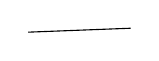
\begin{tikzpicture}\draw (0,0)--(1.3,.05);\end{tikzpicture}}

Ensembles quasi-\unsure{schématiques}.

\unsure{Les ens} \unsure{pro-schématiques} de type fini sur un
\deleted{\unsure{schéma}} \unsure{ens} \unsure{pro-schématique} \uline{\unsure{noethérien}}
\unsure{forment} une \uline{catégorie géométrique} (?)

\figure{\begin{tikzpicture}\draw (0,0)--(0,1);\end{tikzpicture}}
\margin{98}
\margin{\deleted{\unsure{4}}}

\scanpage{100}
\begin{center}- 12 -\end{center}
\margin{n° 285}

se borner au cas où $I$ est un intervalle de \qquad, et comme la proposition est triviale si $I$ est fini, on peut supposer $I=\unsure{\mathbf N|\mathbb N}$. Soit $x_p\in G_p$; l'hypothèse permet de définir par récurrence sur $n\geq p$ une suite $(x_n)_{n\geq p}$ satisfaisant aux conditions $x_n\in G_n$, $f_{n,n+1}(x_{n+1})=x_n$; il est clair alors que si on pose, pour $m<p$, $x_m=f_{mp}(x_p)$ la suite $(x_n)_{n\geq0}=x$ appartient à $G$ et que $f_p(x)=x_p$, d'où la proposition.

PROPOSITION 23 - \uline{Les notations étant celles du cor.1 de la prop.20, on suppose en outre que pour tout} $\alpha\in I$, \uline{l'application canonique} $\varphi_\alpha$ \uline{de} $A$ \uline{dans} $A_\alpha$ \uline{soit surjective}. \uline{Alors, si pour tout} $\alpha\in I$ $g_\alpha(A_\alpha)$ \uline{est dense dans} $B_\alpha$, $g(A)$ \uline{est dense dans} $B$.

En effet, il suffit de montrer que, pour tout $\alpha\in I$ et tout ensemble ouvert non vide $U_\alpha$ dans $B_\alpha$, il existe $x\in A$ tel que $\psi_\alpha(g(x))\in U_\alpha$ (en désignant par $\psi_\alpha$ l'application canonique de $B$ dans $B_\alpha$). Mais par hypothèse il existe $x_\alpha\in A_\alpha$ tel que $g_\alpha(x_\alpha)\in U_\alpha$, et il existe $x\in A$ tel que $\varphi_\alpha(x)=x_\alpha$; comme $\psi_\alpha(g(x))=g_\alpha(\varphi_\alpha(x))$, cet élément répond à la question

PROPOSITION 24 - \uline{Soient} $(G_\alpha,f_{\alpha\beta})$ \uline{un système projectif de groupes topologiques}, $G=\varprojlim G_\alpha$, $f_\alpha$ \uline{l'application canonique de} $G$ \uline{dans} $G_\alpha$. \uline{On suppose que} : 1°) \uline{pour tout} $\alpha\in I$, $f_\alpha$ \uline{est surjective} ; 2°) \uline{pour tout couple d'indices tel que} $\alpha\leq\beta$, $f_{\alpha\beta}$ \uline{est un homomorphisme de} $G_\beta$ \uline{sur} $G_\alpha$. \uline{Dans ces conditions}, $f_\alpha$ \uline{est un homomorphisme de} $G$ \uline{sur} $G_\alpha$.

En effet, soit $V$ un voisinage quelconque de $e$ dans $G$. Il existe un indice $\beta\geq\alpha$ et un voisinage $V_\beta$ de $e_\beta$ dans $G_\beta$ tel que $W=f_\beta^{-1}(V_\beta)$ soit un voisinage de $e$ contenu dans $V$. Comme $f_\beta$ est surjective, on a $V_\beta=f_\beta(W)$, et comme $f_{\alpha\beta}$ est un homomorphisme surjectif, $f_{\alpha\beta}(V_\beta)$ est un voisinage de $e_{\unsure{\alpha}}$ dans $G_\alpha$; mais on a $f_\alpha(W)=f_{\alpha\beta}(f_\beta(W))=f_{\alpha\beta}(V_\beta)$ d'où la proposition (th.1).

Soit $N_\alpha$ le noyau de $f_\alpha$; les $N_\alpha$ constituent une base de filtre, formée

\margin{99}

\scanpage{101}
\deleted{\unsure{Pro-schématiques} \unsure{sur} \unsure{k}}

\diagram{\begin{tikzcd}[ampersand replacement=\&,column sep=large]
(\text{Ens. }\unsure{\text{schématiques}}\text{ }\unsure{\text{sur}}\ k)
\arrow[r,"\text{pl. fidèle}"'] \& \underline{\operatorname{Hom}}((\text{Ens }\unsure{\text{schém.}}/k),(\text{Ens}))
\end{tikzcd}}

\diagram{\begin{tikzcd}[ampersand replacement=\&]
\& X \& \\
S \arrow[ur,dashed,"\unsure{\exists}"] \& S'\arrow[l]\arrow[u] \& S''\arrow[l,shift left]\arrow[l,shift right]
\end{tikzcd}}

\uuline{application surjective}\hfill\uline{\unsure{morphisme} fid. plat}

\uline{Tout épimorphisme est un morphisme de descente}

\[
\left\{\begin{array}{l}
\left[\begin{array}{ll}
1)&\text{Existence de }\varprojlim\text{ finies}\\
2)&\text{Existence du }\unsure{\text{quot}}\text{ par un graphe d'équivalence}
\end{array}\right.\\[4pt]
\left[\begin{array}{ll}
3)&\deleted{\text{Tout}}\ \text{épim est effectif}\\
4)&\text{Tout épim est universel}
\end{array}\right.
\end{array}\right.
\]
\margin{[\unsure{donc ça marche} pour \unsure{principes} d'\unsure{équivalence}\ldots]}

\deleted{5) Tout morphisme se factorise par un \unsure{produit} \unsure{des} [\unsure{épim}, \unsure{monom}]}

\diagram{\begin{tikzcd}[ampersand replacement=\&,column sep=small,execute at end picture={\draw (0.4,0.5) ellipse (2.3cm and 0.9cm);\draw (-2.9,0.25)--(-1.55,0.25);}]
\deleted{\unsure{E}}\arrow[r] \& X\times_Y X\arrow[r,shift left]\arrow[r,shift right] \& X\arrow[r]\arrow[dr] \&Y\\
\&\&\&X'\arrow[u,hook,"\unsure{\text{mon}}"']
\end{tikzcd}}

\[
\left\{\begin{array}{l}
\left[\begin{array}{ll}
1')&\text{Existence de }\varinjlim\text{ finies}\\
2')&\text{Existence du }\unsure{\text{coquotient}}\text{ par un cographe d'équivalence}
\end{array}\right.\\[4pt]
\left[\begin{array}{ll}
3')&\text{Tout mon est effectif}\\
4')&\unsure{\text{Co-changement}}\text{ de base }\unsure{\text{dans un}|\text{d’un}}\text{ monomorphisme}
\end{array}\right.
\end{array}\right.
\]
\margin{?}
\figure{\begin{tikzpicture}\draw (0,4.4) .. controls (.2,3.2) and (1.7,2.8) .. (2.8,2.5) .. controls (3.3,2.1) and (2.7,1.3) .. (2.8,0);\end{tikzpicture}}

\uline{Axiome géométrique}\qquad
$X\times\coprod Y_i\simeq\coprod_i X\times Y_i$

[\unsure{ou aussi}: \unsure{chgt} de base commute aux sommes,
-- donc aux $\varinjlim$ finies ???]

\diagram{\begin{tikzcd}[ampersand replacement=\&]R\arrow[r]\&S\end{tikzcd}}
\figure{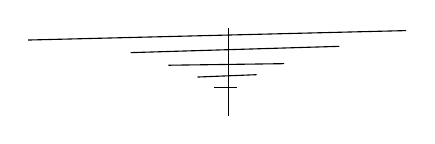
\begin{tikzpicture}[x=1cm,y=1cm]
\draw (-2.4,0)--(2.4,0.12);
\draw (-1.1,-0.16)--(1.55,-0.08);
\draw (-0.62,-0.32)--(0.85,-0.30);
\draw (-0.25,-0.47)--(0.50,-0.44);
\draw (-0.04,-0.60)--(0.25,-0.60);
\draw (0.14,0.15)--(0.14,-0.96);
\end{tikzpicture}}
\margin{100}

\scanpage{102}
\begin{center}- 10 -\end{center}
\margin{n° 285}

topologiques $(G_\alpha)$ et la famille d'applications $(j_\alpha\circ g_\alpha)$, en désignant par $g_\alpha$ l'application canonique de $H$ dans $H_\alpha$. Comme $j_\alpha\circ g_\alpha=f_\alpha\circ j$, le même critère de transitivité prouve que $j$ est un isomorphisme de $H$ sur le sous-groupe $j(H)$. En outre, $j(H)$ est l'intersection, dans le groupe produit $F=\prod_{\alpha\in I}G_\alpha$, de $G$ et du sous-groupe $\prod_{\alpha\in I}H_\alpha$ d'où la dernière assertion du corollaire.

Lorsque les hypothèses du cor.2 sont satisfaites, on dit que $(H_\alpha)$ est un \uline{système projectif de sous-groupes} correspondant au système projectif de groupes $(G_\alpha)$, et on identifie d'ordinaire $H$ et $j(H)$ au moyen de l'injection $j$.

Soit $K$ un sous-groupe de $G=\varprojlim G_\alpha$, et posons $K_\alpha=f_\alpha(K)$ ; il est immédiat que $(K_\alpha)$ est un système projectif de sous-groupes dont la limite projective $H$ s'identifie à un sous-groupe de $G$. Il est clair en outre que $H\supset K$ et on voit aussitôt que $K$ est dense dans $H$ (cf. prop.23) ; mais en général on aura $H\neq K$ (exerc. voir §3, cor.1 de la prop.18).
\margin{\unsure{2|?}}

\uline{Corollaire} 3 - \uline{Les hypothèses et notations étant celles du cor.1, soit} $N_\alpha$ \uline{le noyau de} $g_\alpha$ ; \uline{alors} $(N_\alpha)$ \uline{est un système projectif de sous-groupes distingués, dont la limite projective est le noyau de} $g=\varprojlim g_\alpha$

La relation $g_\alpha\circ\varphi_{\alpha\beta}=\psi_{\alpha\beta}\circ g_\beta$ pour $\alpha\leq\beta$ montre aussitôt que $(N_\alpha)$ est un système projectif. En outre, si $\varphi_\alpha$ (resp. $\psi_\alpha$) est l'application canonique de $A$ dans $A_\alpha$ (resp. de $B$ dans $B_\alpha$), la relation $\psi_\alpha(g(x))=g_\alpha(\varphi_\alpha(x))$ pour $x\in A$ montre que si $x\in N=\varprojlim N_\alpha$, on a $\psi_\alpha(g(x))=e$ pour tout $\alpha\in I$, donc $g(x)=e$, et réciproquement cette dernière relation entraîne $\varphi_\alpha(x)\in N_\alpha$ pour tout $\alpha\in I$, donc $x\in N$. Ce raisonnement montre en outre que $N$ est \uline{l'intersection des sous-groupes} $\varphi_\alpha^{-1}(N_\alpha)$ (qui forment une base de filtre, comme on le vérifie aussitôt).

\margin{101}

\scanpage{104}
\uline{Définition} 1\quad Soit $X$ un espace topologique. On appelle topologie constructible de $X$, \deleted{\unsure{dont}} la topologie dont les ouverts sont les réunions quelconques de parties loc. constructibles [donc une base d'ouverts fournie par les parties loc. constructibles,]. Parties \unsure{antifiques|antifinies} $=$ fermés de $X^{\mathrm{cons}}$ $=$ intersections de parties loc. constructibles.

\margin{\deleted{\unsure{Universel} \illegible{2}}}
\uline{Prop 1}\quad Supposons que \deleted{tout point de} $X$ admette une base \inserted{$(U_i)_{i\in I}$} formée d'ouverts rétrocompacts. Alors

(0) les parties constructibles de $X$ forment une base d'ouverts de $X^{\mathrm{cons}}$

i) La topologie constructible de $X$ est plus fine que la topologie donnée, i.e. $X^{\mathrm{cons}}\unsure{\text{---}|\longrightarrow}X$ est continue.

ii) \deleted{\unsure{Si on}}\inserted{Si} $X$ satisfait de plus $T_0$, alors $X^{\mathrm{cons}}$ est séparé [$=$ tot. discontinu] et réciproquement.

iii) Si $\unsure{E}$ est une \deleted{ouvert de $X$, la topologie}\inserted{partie constructible de $X$,} munie de sa topologie induite $T_E$, alors la topologie constructible $T_E^{\mathrm{cons}}$ associée à $T_E$ est induite par $T^{\mathrm{cons}}$ sur $E$.

\margin{\figure{\begin{tikzpicture}[x=1cm,y=1cm]
\draw (0,0)--(0,-0.65);
\draw (0.20,-1.0)--(0.24,-1.6);
\draw (0.34,-1.95)--(0.42,-2.45);
\draw (0.48,-2.85)--(0.50,-4.15);
\end{tikzpicture}}}

(0) Car un loc. constructible $E$ est réunion des $U_i\cap E$, qui est constructible dans $X$ par $\unsure{0_{\mathrm{III}}|0_{\mathrm{II}}}$ 9.1.8.

i) Résulte du fait que les $U_i$ sont \inserted{[loc]} constructibles, donc ouverts pour $T_{\unsure{X}}^{\mathrm{cons}}$. Pour ii), \deleted{\unsure{soit}}, $x,y\in X$, il existe un \unsure{des deux, soit} $x$, et un voisinage ouvert $U\ni x$, $U\not\ni y$. On peut grâce à l'hyp supposer $U$ rétrocompact, donc [loc.] constructible, et $X-U=V$ l'est \inserted{alors} également, alors
\[
U\cap V=\varnothing,\quad U\cup V=X,\quad U\ni x,\quad V\ni y,\quad U,V\text{ ouverts pour }T_{\unsure{E|X}}.
\]

Pour iii), on sait que la topologie induite par $T_{\unsure{X|E}}^{\mathrm{cons}}$ sur $E$ a comme base d'ouverts les $E\cap F$, $F$ \deleted{\unsure{co}}\inserted{loc}. constructible dans $X$, ce sont exactement les $G\subset E$ loc. constructibles dans $E$,

\margin{103}

\scanpage{105}
grâce au

\uline{Lemme}\quad a) Soit $\unsure{E|F}$ (loc.) constructible dans $X$, \inserted{($E$ loc. const.)} alors $F\cap E$ est (loc) constructible dans $E$

b) Soit $F\subset E$, \inserted{avec $E$ (loc) constructible} alors $F$ est (loc.) const. dans $E$ ssi il l'est dans $X$.

\margin{\figure{\begin{tikzpicture}\draw (0,0)--(0,-0.5);\draw (0.1,-1.1)--(0.15,-1.55);\end{tikzpicture}}}

Dém. Pour a), on montre que si $F$ est ouvert rétrocompact dans $X$, alors $F\cap E$ est rétrocompact dans $E$, grâce au fait que \unsure{$\forall$} ouvert quasi cpt $U$ de $E$ est induit par un ouvert $V$ de $X$, qu'on peut \unsure{si on veut} [grâce à l'hyp préliminaire de la prop] supposer quasi cpt, d'où
\[
f^{-1}(F)\cap U=f^{-1}(F\cap V)=\text{image inverse}
\]
d'un quasi cpt, qui est quasi cpt car $E$ est rétrocompact dans $X$, \inserted{par $\unsure{0_{\mathrm{III}}}$ 9.1.13.} \deleted{Donc} Le cas ``localement'' en résulte aussitôt, utilisant le fait que $E$ induit un $E\cap U$ constructible dans \deleted{\unsure{tt}} $U$ ouvert.

\margin{\diagram{\begin{tikzcd}[ampersand replacement=\&,column sep=small,row sep=small]
E\arrow[d,"f"']\& f^{-1}(F)\cap U\\
X\&F
\end{tikzcd}}}

Pour b), on suppose $F\subset E$ constructible dans \uline{$E$}, \inserted{construct.} prouvons que $F$ l'est dans $X$. On peut supposer $F$ \deleted{\unsure{ouvert}}\inserted{\deleted{fermé}\inserted{ouvert}} dans $E$, rétrocompact dans $E$, \deleted{et}\inserted{\unsure{puis: on}} $E=U\cap\complement V$, $U$ et $V$ rétrocomp. dans $X$ \inserted{\unsure{qui sont constructibles}}

[car $E=\bigcup E_i$ réunion finie de tels, les \deleted{$F\cap E_i$ est} dans \uline{$E$} par a), donc $E_i\cap F$ const. dans $E_i$ par a), et on est ramené à prouver qu'ils sont constructibles dans $X$, puisque $F=\bigcup E_i\cap F$.

\margin{$\unsure{0_{\mathrm{III}}}$ 9.1.8 \unsure{(i)(ii)}}

\inserted{Remplaçant $X$ par $U$, on peut supposer $E$}
\deleted{On suppose $F$ est \unsure{ouvert} dans $E$, \illegible{2}}
\inserted{\unsure{se borne au cas} $X=U$}
\deleted{$F=E\cap W$, $W$ \unsure{ouvert} dans $X$, \illegible{2}}
\margin{[$E$ étant const. dans $U$, $F$ \inserted{(par ii)} \unsure{le sera} dans $U$, donc dans $X$]}

\figure{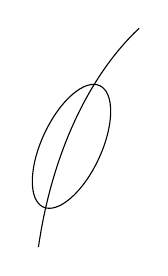
\begin{tikzpicture}[x=1cm,y=1cm]
\draw[rotate=-25] (0,0) ellipse (0.38cm and 0.85cm);
\draw (-0.42,-1.28)..controls(-0.25,-0.1)and(0.22,0.9)..(0.86,1.5);
\end{tikzpicture}}
\margin{104}

\scanpage{106}
Donc on peut supposer $E=\complement V$, $V$ \deleted{est} ouvert rétrocompact,
\deleted{et par suite on aura $\unsure{E-F}=F=\complement\unsure{U}$ \unsure{le cas}}, Il suffit de prouver \inserted{\unsure{le puis}} $E-F$ const. dans $X$, i.e.
\[
X-(E-F)=V\cup F\text{ rétrocompact dans }X,
\]
ce qui est le cas car $V$ et $F$ le sont évidemment.

\margin{\diagram{\begin{tikzcd}[ampersand replacement=\&,row sep=small]
\complement V\arrow[d,no head]\vphantom{F}\\[-1ex]
\unsure{F}\arrow[d,no head]\\[-1ex]
\unsure{\cdot}
\end{tikzcd}}}

Le cas ``local'' résulte aussitôt du cas global.

\uline{Corollaire} 1\quad Supposons que de plus, \unsure{$\forall$} partie $U_i$ soit \uline{quasi compacte} \deleted{\unsure{fermée}} \uline{pour la topologie constructible} [donc aussi \deleted{pour la top} compacts pour la top constructible, dans le cas où \deleted{\unsure{la top}} $X$ satisfait $(T_0)$], \inserted{i.e. \unsure{satisfaisant} à la condition: $\unsure{\#}\ \unsure{---}\ \unsure{!}$} Alors

iv) Les $U_i^{\mathrm{cons}}$ sont quasi-compacts, \deleted{et $X$ \unsure{est donc}}
\deleted{\unsure{ouvert} \unsure{quasi} \unsure{cpt} une base formée d'ouverts}
\deleted{\unsure{pour} $X$ \unsure{admet} une base formée d'ouverts}

(v) Soit $E$ une partie \deleted{loc. constructible de}\inserted{fermée de} $X^{\mathrm{cons}}$ [p.ex. une partie loc. constructible de $X$] alors
\[
\begin{aligned}
E\ \deleted{\text{compact}}\ \text{quasi-compact}\ \inserted{\unsure{\text{(fort. q.cpt)}}}\ \text{dans }X^{\mathrm{cons}}
&\Longleftrightarrow E\text{ quasi-compact dans }X\\
&\Longleftrightarrow E\subset\text{réunion finie des }U_i.
\end{aligned}
\]

(vi) Pour que $X^{\mathrm{cons}}$ soit loc. cpt [cpt] il f. et s. que $X$ satisfasse $(T_0)$ [resp. $(T_0)$, et soit q. cpt].

\margin{N.B. Les hypothèses faites impliquent que \unsure{tt} fermé irred. de $X$ \unsure{admet} un \deleted{\unsure{pt}} pt générique (\unsure{compte tenu de} $T_0$ \unsure{est réciproque|et réciproque}\unsure{---})}

\margin{\figure{\begin{tikzpicture}[x=1cm,y=1cm]
\draw (0,0)--(0.12,-1.7);
\draw (0.2,-2.0)--(0.23,-2.7);
\draw (0.3,-3.1)--(0.38,-5.2)--(0.58,-5.22);
\end{tikzpicture}}}

(iv) Résulte de (i) trivialement. Évident
\[
E^{\mathrm{cons}}\text{ q. cpt}\Longrightarrow E\text{ q. cpt en vertu de (i)}
\]
$\Longrightarrow E\subset$ union finie \inserted{$V$} des $U_i$ par définition de q. cpt, donc $E$ fermé dans $V^{\mathrm{cons}}$ [pour la top. induite par $X^{\mathrm{cons}}$] qui est aussi $\bigcup U_i^{\mathrm{cons}}$, et les $U_i^{\mathrm{cons}}$ sont q. cpt, donc $E$ l'est, C.Q.

\margin{(vi) En résulte trivialement}
\margin{105}

\scanpage{107}
\uline{Corollaire} 2\quad \deleted{Dans les conditions du corollaire 1} Supposons $X$ \deleted{\unsure{de plus}} quasi compact, \inserted{et $(T_0)$} et que \deleted{\unsure{toute partie}} $X$ ait une base formée d'ouverts \deleted{\unsure{quasi compacts}} rétrocompacts, qui sont q. cpts pour la topologie constructible. Soit $E$ une partie de $X$. Conditions équivalentes

a) $E$ est fermé pour la top. constructible [i.e. est intersection \deleted{finie} de parties constructibles]

b) $E$ est compact pour la top constructible, i.e. pour \unsure{$\forall$} famille de parties constructibles $(E_i)_{i\in I}$ de $X$, telle que $E\subset\bigcup_{i\in I}E_i$, il existe une sous-famille finie $J\subset I$, telle que $E\subset\bigcup_{i\in J}E_i$.

\margin{en général, \uline{partie \unsure{antifique|antifinie}} $=$ \uline{intersection de loc constructibles}. \unsure{Nature locale de la notion} ??}

\deleted{$X$ \unsure{est}} En effet, $X^{\mathrm{cons}}$ est compact, donc a) $\Longleftrightarrow$ b).

On est \unsure{convenu}\inserted{alors} que \deleted{\unsure{E}} $E$ est une \uline{partie \unsure{antifique|antifinie} de} $X$. On peut donner un énoncé analogue si $X$ n'est plus supposé q. cpt [mais satisfaisant aux deux hyp]

\diagram{\begin{tikzcd}[ampersand replacement=\&,row sep=large]
\begin{gathered}E\text{ fermé}\ \inserted{\text{dans }X^{\mathrm{cons}}}\\
[\text{i.e. intersection de parties loc. constructibles}]
\end{gathered}\arrow[d,Leftrightarrow]\\
\begin{gathered}
E\text{ loc. cpt pour la top. constructible i.e. pour }\unsure{\forall}\\
\deleted{\text{partie }\unsure{\forall}}\ U_i,\quad E\cap\unsure{U_i}\text{ satisfait la condition b}\\
\text{ci-dessus dans }U_i.
\end{gathered}
\end{tikzcd}}

\uline{Corollaire} 3\quad Dans les conditions du corollaire 2, Conditions équivalentes

a) $E$ et $X-E$ sont \unsure{antifiques|antifinies}

b) $E$ est \deleted{constructible} ouvert et fermé dans $X^{\mathrm{cons}}$

c) $E$ est constructible.

\margin{\figure{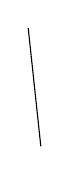
\begin{tikzpicture}\draw (0,0)--(0.16,-1.5);\end{tikzpicture}}}
\margin{106}

\scanpage{108}
$c\Longrightarrow a)\Longleftrightarrow b)$ trivial, pour la réciproque $a\Longrightarrow c$, noter que $E$ et $X-E=F$ étant ouverts dans $X^{\mathrm{cons}}$, sont réunions \deleted{d'ouverts} \deleted{\unsure{d'ens}} filtrantes d'ens constructibles $E_i$ resp. $F_j$, et $X$ est réunion filtrante des $E_i\cup F_j$, donc est égal à l'un des $E_i\cup F_j$, d'où $E=E_i$, \deleted{$\unsure{E\subset F_j}$} $F=F_j$ pour un $i,j$, donc $\unsure{E_i,F_j|E,F}$ constructibles.

\uline{Proposition 2}\quad Soit $f:X\longrightarrow Y$ une application continue d'espaces topologiques, telle que \deleted{\unsure{si}} pour \unsure{$\forall$} couple d'ouverts $V\subset U\subset Y$, \deleted{rétrocompact dans $Y$}\inserted{$V$ rétrocompact dans $U$}, $f^{-1}(\unsure{U|V})$ soit rétrocompact dans $f^{-1}(U)$. Alors

\margin{hyp. \unsure{trop restrictive} pour un \unsure{morphisme} de \unsure{préschémas}}

\deleted{(0) Pour \unsure{$\forall$} \unsure{immers} $Y'$ de $Y$ posons $X'=f^{-1}(Y')$, $f':X'\longrightarrow Y'$ satisfait \unsure{les mêmes hyp}.}

\unsure{(i)} Pour \unsure{$\forall$} partie constructible [loc. constructible] \deleted{\unsure{en}} $\unsure{E}$ de $Y$, $f^{-1}(\unsure{E})$ est une partie constructible [loc. constructible].

(ii) $f$ est continue de $X^{\mathrm{cons}}$ en $Y^{\mathrm{cons}}$, i.e. l'image inverse d'une partie \inserted{\deleted{loc.}} \unsure{antifique|antifinie} de $Y$ est une partie \inserted{loc.} \unsure{antifique|antifinie} de $X$.

\margin{$Y'\subset Y$}

\inserted{\unsure{car}} (i) est trivial pour ``constructible''. Pour loc. constructible, on utilise qu'on aura $Y=\bigcup Y_i$, les $Y_i$ ouverts, les $E_i=E\cap Y_i$ constructibles \inserted{dans $Y_i$}, Alors $X_i=f^{-1}(Y_i)$, \inserted{$f_i:X_i\longrightarrow Y_i$ induit,} il suffit de prouver que $f_i^{-1}(E_i)$ sont constructibles dans $X_i$, donc de prouver que $X_i\underset{\inserted{f_i}}{\unsure{-|\longrightarrow}}Y_i$ satisfait l'hyp. de $f:X\longrightarrow Y$, \deleted{c'est} Cl.

ii) Résulte trivialt de i).

\margin{107}

\scanpage{109}
\deleted{\uline{Corollaire 1}\quad Supposons que dans $X$ et $Y$, \deleted{\unsure{tt pt}} \deleted{\unsure{admettent} \unsure{une|un} \unsure{système|application} \unsure{fondamental} de \unsure{vois.}}\inserted{base d'ouverts \inserted{$X_i$ resp. $Y_j$} rétrocompacts quasi-compacts}. Alors l'hyp préliminaire de la prop. équivaut aussi à dire que Pour \unsure{$\forall$} ouvert \deleted{\unsure{quasi}} $Y_j$, $f^{-1}(Y_j)$ est rétrocompact dans $X$, ou encore que pour \unsure{$\forall$} \deleted{ouvert} ouvert $Y'$ \deleted{quasi cpt}\inserted{\deleted{\unsure{E rétrocompact}} rétrocompact} de $Y$, $X'=f^{-1}(\unsure{Y'|U'})$ est \deleted{q. cpt} rétrocompact dans $X$, ou encore que les $X_i\cap f^{-1}(Y_j)$ sont q. cpts.}

[\uline{Prop.} Soit $X$ un espace topologique, ayant une base d'ouverts $U_i$ qui sont quasi-compacts. Alors pour \unsure{$\forall$} \deleted{partie $E$ de $X$, il revient} application continue $f:X'\unsure{-|\longrightarrow}X$, il revient au même de dire que $f$ est q. cpt, ou que les $f^{-1}(U_i)$ sont q. cpts.

Donc si $X'\subset X$ sous-espace top. $X'$ est rétrocompact dans $X$ ssi les $X'\cap U_i$ sont q. cpts.

\uline{Cor.} \deleted{Soit \unsure{Supposons} de plus}\inserted{Pour que} les $U_i$ rétrocompacts dans $X$, \deleted{Alors}\inserted{il f. et s. que} \uline{\unsure{$\forall$}} partie quasi-compacte ouverte de $X$ soit rétrocompacte dans $X$.

\margin{\deleted{\uline{Cor} b) $f:X'\unsure{-|\longrightarrow}X$ q. cpt \unsure{dans} $X$ \illegible{2}}}

\uline{Cor.} S'il en est ainsi, pour une \deleted{\unsure{ap}} applic. continue $f:X'\unsure{-|\longrightarrow}X$, il revient au même de \unsure{dire} \unsure{conditions}

(a) pour \unsure{$\forall$} $U\subset X$ \inserted{ouvert} qui est rétrocompact, $f^{-1}(U)$ est rétrocompact,

(b) Pour \unsure{$\forall$} $U_i$, $f^{-1}(U_i)$ est rétrocompact dans $X'$,

(c) [Si $X'$ a une base d'ouverts quasi-compacts $U'_j$] les $f^{-1}(U_i)\cap U'_j$ sont \deleted{rétro} qua cpts.]

\margin{$U\subset X$ ouv. rétrocompact, si $U'\subset X'$ ouv. q. cpt}
\margin{$b\Rightarrow a$, En effet, $f^{-1}(U)\cap\unsure{V'|U'}\subset f^{-1}(f(U'))$, \deleted{$=f^{-1}(U)\cap\unsure{f^{-1}}$}, et $f(U')$ étant q. cpt, est contenu dans une réunion finie de $U_i$ $(i\in J)$, donc
\[
f^{-1}(U)\cap V'=f^{-1}\left(\bigcup_{i\in J}U\cap U_i\right)\cap V'.
\]
Or chaque $U\cap U_i$ est réunion finie \unsure{d'uns} $U_j$}

\margin{\figure{\begin{tikzpicture}[x=1cm,y=1cm]
\draw (0,0)--(0.15,-2.1);
\draw (0.3,-4.5)..controls(0.3,-5.1)and(0.7,-5.1)..(1.5,-5.2)..controls(2.7,-5.25)and(3.1,-5.5)..(3.35,-5.9);
\end{tikzpicture}}}
\margin{108}

\scanpage{110}
\uline{Corollaire 1}\quad Supposons que $X$, \inserted{$Y$} \deleted{\unsure{soient des}} \inserted{soient} des espaces $T_0$, \deleted{\unsure{élémentaires qui}} admettant des bases d'ouverts formées d'ens \deleted{quasi-cpts} rétrocompacts et q. cpts pour la top. constructible [donc compacts pour la dite], \deleted{\unsure{lesquels}} \inserted{Conditions} équivalentes:

a) $f:X\longrightarrow Y$ \deleted{soit} \deleted{\unsure{une telle que}} \inserted{est} quasi-compacte

\deleted{[\unsure{si} cpt $X$}\quad \deleted{Alors} b) $f^{\mathrm{cons}}$ est une \deleted{application} application propre d'espaces loc. cpts \deleted{c) \unsure{les} $f(\unsure{X_i})$ \unsure{parties} $X\subset f$}.

\deleted{[\unsure{les} $f$ transforme parties \unsure{antifiques|antifinies} en parties \unsure{antifiques|antifinies}]}

\margin{c) $f$ transforme parties \unsure{antifiques|antifinies} en parties \unsure{antifiques|antifinies}, et les fibres de $f$ sont quasi-compactes [\unsure{après}: Bourbaki, Top \deleted{\unsure{II}} I, \unsure{10,2,th.1}]}

[NB. $f$ en particulier transforme les parties constructibles en parties constructibles, \deleted{et \unsure{bien les cas fermés} \inserted{\unsure{plus loc}} \unsure{est fermé}, \unsure{cela est transforme les}}]

\uline{Corollaire 2}\quad Sous les conditions précédentes \inserted{\unsure{les vérifier}}, supposons $Y$ et $X$ quasi cpts, donc $X^{\mathrm{cons}}$, $Y^{\mathrm{cons}}$ \uline{compacts}. Conditions équivalentes

a) $f$ transforme parties constructibles en parties constructibles [i.e. transforme ``ouverts et fermés'' en ``ouverts et fermés'']

b) $f$ transforme parties constructibles en parties réunions de constructibles [i.e. ``ouverts et fermés'' en ``ouverts'']

(c) $f^{\mathrm{cons}}$ est une application \uline{ouverte}. \deleted{\unsure{(qui est propre)}}

Ces conditions sont vérifiées si $f$ est \uline{bijective}.

\uline{Cor. 3}\quad Si les conditions du lemme 1 sont remplies, alors (i) $f(X)$ est \unsure{antifique|antifinie}; (ii) pour \unsure{$E\subset Y$}, une partie \inserted{$E$} de $f(X)$ est \unsure{antifique|antifinie} ssi $f^{-1}(E)$ l'est (iii) Si $f$ est surjective, une partie de $Y$ est constructible ssi $f^{-1}(\unsure{Y|E})$ l'est.

\margin{\figure{\begin{tikzpicture}[x=1cm,y=1cm]
\draw(0,0)--(.12,-5.0);
\draw(0,-6.0)..controls(.1,-7.8)and(-.3,-11.0)..(.4,-11.3);
\end{tikzpicture}}}
\margin{109}

\scanpage{111}
Examinons \unsure{un peu} de près les parties \unsure{antifiques|antifinies} \inserted{(et loc. constructibles)} de $X$, quand on ne suppose pas $X$ q. cpt. .....

\figure{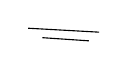
\begin{tikzpicture}[x=1cm,y=1cm]\draw(0,0)--(.9,-.05);\draw(.18,-.12)--(.77,-.16);\end{tikzpicture}}

\uline{\unsure{Pr.}} Soit $X$ un schéma affine. Alors $X^{\mathrm{cons}}$ est compact.

\uline{Corollaire 1} Soit $X$ un préschéma \deleted{\unsure{quelconque|noethérien}} \inserted{q. séparé}. Alors $X$ est $T_0$, admet une base formée d'ouverts rétrocompacts et compacts pour la topologie constructible. En partic., $X^{\mathrm{cons}}$ est loc. compact.

\uline{Corollaire \unsure{2|3}} Supposons \deleted{de plus} $X$ [quasi-compact et quasi-séparé] \deleted{Alors} quasi-noethérien. Alors

(i) $X^{\mathrm{cons}}$ est compact. (ii) les parties constructibles de $X$ sont les parties ouvertes et fermées de $X^{\mathrm{cons}}$.

(iii) les parties \deleted{\unsure{affines et}} \unsure{antifiques|antifinies} de $X$ sont les parties $E$ telles qu'il existe un morphisme q. cpt $f:X'\longrightarrow X$ d'image $E$.

On peut prendre \inserted{pour} \deleted{\unsure{$f$}} $X'\longrightarrow X$ un \uline{monomorphisme} q. cpt \unsure{...}

\deleted{[NB. \unsure{admet}} (iv) Si $E$ et $X-E$ ont cette propriété, ils sont constructibles ....

\margin{\figure{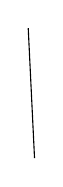
\begin{tikzpicture}[x=1cm,y=1cm]\draw(0,0)--(.08,-1.65);\end{tikzpicture}}}
\margin{110}

\scanpage{113}
Soient $X,Y$ deux préschémas. \uline{Applications géométriques} de $E\subset X$ en $Y$: morphismes de $\operatorname{Dis}(\unsure{E;X})=\coprod_{x\in E}\operatorname{Sp}k(x)$ vers $\operatorname{Dis}(Y)$. \inserted{Supposons $E$ loc. constructible} Une application géométrique est dite \uline{constructible} si \unsure{tt} $x\in X$ a un voisinage ouvert \inserted{affine} $U$, et une partition de $U\cap E$ en parties loc. fermées $Z_i$, telle que $f\mid(Z_i)_{\mathrm{red}}$ soit un \uline{morphisme} $Z_i\longrightarrow Y$. \deleted{Il revient au même de dire que}

Ex: une appl. géom. définie par un morphisme. Si on a $E=\bigcup_{i\in I}E_i$ \unsure{famille} \uline{quelconque} de parties loc. constructibles, alors $f:E\mathrel{\overset{\text{appl. géom.}}{\unsure{-|\longrightarrow}}}Y$ est constr. ssi pour \unsure{$\forall$} $i$, $f\mid E_i$ l'est; cela signifie aussi, \inserted{si $\unsure{X|E}$ est quasi-compact et q. sép.} qu'on peut trouver une \uline{partition} globale de $E$ en parties $Z_i$ constructibles loc. fermées, telles que les $f\mid Z_i$ soient des morphismes. / Définition de $\operatorname{App}_{\mathrm{cons}}((X,E),(\unsure{Y|X},F))$, Transitivité.

\unsure{Ctégorie} \inserted{$(\mathrm{Cons\ Aff})$} des modèles constructibles affines: objets les schémas affines (ou si on préfère, quasi-compacts q. sép.) et morphismes les appl. constructibles. Si $E$ est une partie loc. \deleted{\unsure{préschéma, ou bien}} constructible d'un préschéma $X$, on lui associe un foncteur
\[
\operatorname{Cons}(\unsure{X|Z},E):(\mathrm{Cons\ Aff})^\circ\longrightarrow(\mathrm{Ens})
\]
\margin{112}

\scanpage{114}
Par
\[
\operatorname{Cons}(X,E)(Y)=\operatorname{App}_{\mathrm{cons}}(Y,(X,E))
\]
\deleted{\unsure{On a}}

Si on a $(X,E)$ et $(X',E')$, on a.
\[
\operatorname{App}_{\mathrm{cons}}((X,E),(X',E'))\xrightarrow{\sim}\operatorname{Hom}(\operatorname{Cons}(X,E),\operatorname{Cons}(X',E'))
\]
On obtient ainsi des foncteurs pleinement fidèles

\diagram{\begin{tikzcd}[ampersand replacement=\&,column sep=large,row sep=huge]
(\mathrm{Cons\ Aff})
 \arrow[r]
 \arrow[r,bend left=42,"{\substack{\text{\unsure{épimorphismes|morphismes les}}\\\text{\unsure{cons. définies par q. cpts}...}}}"]
 \arrow[rr,bend right=35,"{\text{canonique}}"']
 \arrow[rrr,bend right=58,"{\text{can}}"']
\& \begin{gathered}(\text{Couples }(X,E))\\\text{$E$ loc. constr.}\\\text{dans $\unsure{X|E}$ quasép}\end{gathered}
 \arrow[r]
\& \underbrace{\operatorname{Ind}(\mathrm{Cons\ Aff})'}_{\substack{\text{systèmes}\\\text{inductifs}\\\text{\unsure{immersifs}---}}}
 \arrow[r]
 \arrow[r,bend right=40,"{\text{can}}"']
\& \underline{\operatorname{Hom}}((\mathrm{Cons\ Aff})^\circ,\unsure{\mathrm{Ens}})
\end{tikzcd}}
\margin{113}

\scanpage{115}
Soit $A$ un anneau commutatif, $X$ le schéma affine qu'il définit,
\[
A^{\mathrm{cons}}=\underset{\unsure{\mathfrak P|\mathcal P}}{\unsure{\underline{\lim}|\varinjlim}} A_{\unsure{\mathfrak P|\mathcal P}}
\]
$\unsure{\mathfrak P|\mathcal P}$ parcourt les ``partitions \unsure{ordinaires} de $X$ en ens constructibles loc. fermés, affines, et pour une telle $\unsure{\mathfrak P|\mathcal P}=(X_i)_{i\in I}$, $A_{\unsure{\mathfrak P|\mathcal P}}$ désigne \deleted{\unsure{le produit}} $A(\coprod X_{i\,\mathrm{red}})=\prod A(X_{i\,\mathrm{red}})$.

Les \unsure{hom.} de transition sont injectifs. Considérons
\[
\widetilde X=\operatorname{Spec}(A^{\mathrm{cons}})
\]
On a
\[
\operatorname{Top}(\widetilde X)=\mathop{\underleftarrow{\mathrm{Lim}}}_{\unsure{\mathfrak P|\mathcal P}}\operatorname{Top}\operatorname{Sp}(A_{\unsure{\mathfrak P|\mathcal P}})
\]
En particulier
\[
\operatorname{Ens}(\widetilde X)=\mathop{\underleftarrow{\mathrm{Lim}}}_{\unsure{\mathfrak P|\mathcal P}}\underbrace{\operatorname{Ens}\operatorname{Sp}A_{\unsure{\mathfrak P|\mathcal P}}}_{\coprod X_i}
\]
et comme les morphismes de transition sont des \deleted{\unsure{isomorphismes}} \inserted{bijections}, on trouve \deleted{\unsure{par}} une \deleted{\unsure{surj}} \inserted{bijection}.
\[
\operatorname{Ens}\widetilde X\simeq\operatorname{Ens}X
\]
Cette bijection est compatible avec les topologies de $\widetilde X$ et celle de $X^{\mathrm{cons}}$, comme on voit aisément sur la description d'une base d'ouverts de $\widetilde X$ ....
\margin{114}

\scanpage{116}
\mspage{\unsure{142|146}}
\deleted{Soit $X$ un espace topologique, \deleted{dont chaque \unsure{pt} a un syst. fondamental de voisinages} \inserted{ayant une base d'ouverts} $U$ ayant les propriétés suivantes:

(i) $U$ rétrocompact dans $X$, et $U$ quasi-cpt

(ii) Toute \deleted{suite} famille $(E_i)_{i\in I}$ de parties \deleted{fermées} constructibles de $U$, recouvrant $U$, il y a une sous-famille finie recouvrant $U$.

Pour exprimer (ii), Introduisons [sur \unsure{tt} espace topologique $U$] la topologie dont les ouverts sont les \inserted{réunions quelconques de} parties loc. constructibles [c'est bien stable par intersections finies et réunions qlc] donc une base d'ouverts formée des parties constructibles. Lorsque $U$ est quasi-compact, et que \deleted{\unsure{tt pt admet}} admet une base d'ouverts rétrocompacts, ``loc. constructible'' est d'ailleurs pareil que ``constructible''; moyennant (i), les $U$ \unsure{retrouvent les} \unsure{(Hyp)} \unsure{donnant} dans le cas précédent.

NB. Si de plus $X$ satisfait l'axiome $T_0$, \inserted{[c'est le cas des préschémas]} \deleted{Alors} alors une telle topol. est \uline{séparée}, et même totalement discontinue [pour deux pts $x\ne y$, il existe des ouverts $V\ni x$, $W\ni y$, $V\cap W=\varnothing$, $V\cup W=U$]. L'Hyp (ii) exprime qu'elle est \uline{quasi-compacte} [donc \uline{compacte} dans le cas particulier que nous envisageons].}

\margin{\figure{\begin{tikzpicture}[x=1cm,y=1cm]
\draw(0,0)--(.04,-2.15);
\draw(0,-5.3)ellipse(.15 and .2);\fill(0,-5.3)circle(.025);\draw(-.18,-5.56)--(.22,-5.06);
\end{tikzpicture}}}
\margin{115}

\scanpage{118}
\uline{N\textsuperscript{o} 1}\quad \unsure{Préschémas} cpts et loc. cpts. Anneaux flasques.

\uline{N\textsuperscript{o} 2}\quad \deleted{Systèmes projectifs}\inserted{Proschémas} flasques \deleted{\unsure{proschémas} et \unsure{espaces schématiques} \illegible{2} \unsure{flasques}}

espaces schématiques compacts

\uline{N\textsuperscript{o} 3}\quad \deleted{Espaces \unsure{indschématiques} \unsure{Ind-compacts}} Espaces schématiques.

[Catégorie \unsure{recollable} pour \deleted{\unsure{tous}} les rec. ouverts...]

\margin{Morphismes \unsure{quasi-compacts} \unsure{projectifs} propres}

\uline{N\textsuperscript{o} 4}\quad Opérations sommes, \deleted{\unsure{lim}} et $\underleftarrow{\lim}$ \deleted{finies} des espaces schématiques

\inserted{\unsure{cas non quasi-compact $=$ réunion des compacts}}

\uline{N\textsuperscript{o} 5}\quad \deleted{\unsure{Ens quasi} \unsure{schématiques}} Espaces quasi-schématiques .....

\deleted{\diagram{\begin{tikzcd}[ampersand replacement=\&,column sep=large]
\left(\begin{gathered}\text{Préschémas quasi-compacts}\\\text{quasi-séparés}\end{gathered}\right)
 \arrow[r,"\alpha"]
\&\left(\begin{gathered}\text{Esp. schématiques}\\\text{compacts}\end{gathered}\right)
 \arrow[r,"{\substack{\text{\unsure{équiv.}}\\\deleted{\text{\unsure{naturelle}}}\\\simeq}}"]
\&\left(\operatorname{Pro}(\mathrm{Sch})\ \inserted{\unsure{\lim}}\ \deleted{\unsure{\mathrm{finis}}}\ \text{q. cpts}\right)
 \arrow[r,"{\substack{\unsure{\gamma}\\\text{fid,}\ \deleted{\text{\unsure{surjectif}}}\\\inserted{\text{\unsure{submersif}}}}}"]
\&\left(\begin{gathered}\text{schémas compacts}\\\text{réduits}\end{gathered}\right)
 \arrow[l,bend left=30,"{\sigma\quad\text{pl. fid.}}"']
 \arrow[lll,bend left=40,"{\deleted{\text{\illegible{1}}}\quad\text{pl. fid.}}"']
\end{tikzcd}}}

\uline{N\textsuperscript{o} 6}\quad Pb à \unsure{poser}. Espaces de Néron!

\diagram{\begin{tikzcd}[ampersand replacement=\&,column sep=huge]
\begin{gathered}(\text{Préschémas quasi-compacts}\\\text{quasi-séparés})\\X\end{gathered}
 \arrow[r,"\alpha","{\substack{\text{\unsure{submersif}}\\\text{[fidèle modulo}\\\text{\unsure{nilpotents}].}}}"']
 \arrow[rr,bend left=35,"\sigma"]
\&\begin{gathered}(\mathrm{Cons\ cpt})\\\text{''}\\(\operatorname{Pro}(\mathrm{Sch})\ \text{flasques})\\\mathcal Y\end{gathered}
 \arrow[r,"{\beta=\underleftarrow{\lim}}","{\substack{\text{\unsure{submersif}}\\\text{fidèle}}}"']
\&\begin{gathered}(\text{schémas compacts}\\\text{réduits})\\K\end{gathered}
 \arrow[l,bend left=35,"{\beta'\quad\text{pl. fidèle}}"']
 \arrow[ll,bend left=48,"{\sigma'\quad\text{pl. fid.}\quad\unsure{\text{imm. ouv.}}}"']
\end{tikzcd}}

\margin{$\unsure{\rho|\sigma}$ [pleinement fidèle quand on est ``de type fini'' sur un anneau fixé....]}

\margin{$\beta'(K)=$ système proj. trivial défini par $K$}

\[
\operatorname{Hom}(K,\sigma X)\xrightarrow{\sim}\operatorname{Hom}(\sigma'K,X)
\]
\[
\operatorname{Hom}(K,\beta\mathcal Y)\xrightarrow{\sim}\operatorname{Hom}(\beta'K,\mathcal Y)
\]
\[
\operatorname{Hom}(K,\beta(\alpha X))=\operatorname{Hom}(\beta'K,\alpha X)
\]
\margin{117}

\scanpage{119}
\begin{center}- 90 -\end{center}
\margin{n\textsuperscript{o} 371}

tout $i$. Montrons que l'on a $(u(x))^2=0$ pour tout $x\in M$; on peut en effet écrire $x=\sum_{i=1}^n x_i$, où $x_i\in M_i$, donc $(u(x))^2=\sum_{i=1}^n(u(x_i))^2+\sum_{i<j}(u(x_i)u(x_j)+u(x_j)u(x_i))$.

Or, comme $\psi_i(x_i)$ est un élément de degré 1 dans $\bigwedge(M_i)$, on a, pour $i\ne j$, $h_i(\psi_i(x_i))h_j(\psi_j(x_j))=-h_j(\psi_j(x_j))h_i(\psi_i(x_i))$ (§ 3, n\textsuperscript{o} 3, prop.2), d'où $u(x_i)u(x_j)+u(x_j)u(x_i)=0$; par ailleurs $(u(x_i))^2=h_i((\psi_i(x_i))^2)=0$ par définition de $\bigwedge(M_i)$. En vertu de la prop.3 du n\textsuperscript{o} 2, il existe donc un homomorphisme unique d'algèbres graduées $h:\bigwedge(M)\longrightarrow{}^{\unsure{\mathrm g|\mathrm s}}\!\bigotimes_i(\bigwedge(M_i))$ tel que $u=h\circ\psi$ (où $\psi:M\longrightarrow\bigwedge(M)$ est l'injection canonique). Pour $x_i\in M_i$, on a $h(g(u_i(x_i)))=h(g(h_i(\psi_i(x_i))))=h(f_i(\psi_i(x_i)))=h(\psi(j_i(x_i)))=u_i(x_i)$, et comme les $u_i(x_i)$ engendrent l'algèbre ${}^{\unsure{\mathrm g|\mathrm s}}\!\bigotimes_i(\bigwedge(M_i))$, $h\circ g$ est l'identité; de même $g(h(\psi(j_i(x_i))))=g(u_i(x_i))=g(h_i(\psi_i(x_i)))=f_i(\psi_i(x_i))=\psi(j_i(x_i))$, et les éléments $\psi(j_i(x_i))$ engendrent l'algèbre $\bigwedge(M)$, donc $g\circ h$ est l'identité.

COROLLAIRE 1.- \uline{Sous les hypothèses de la prop.7}, \uline{pour tout entier} $m\geq0$, \uline{la puissance extérieure m-ème} $\mathop{\bigwedge}\limits^m M$ \uline{s'identifie canoniquement par} $g$ \uline{à la somme directe des modules} $\bigotimes_{1\leq i\leq n}(\mathop{\bigwedge}\limits^{m_i}M_i)$, \uline{où} $(m_i)_{1\leq i\leq n}$ \uline{parcourt l'ensemble des suites d'entiers} $\geq0$ \uline{telles que} $\sum_{i=1}^n m_i=m$.

Cet isomorphisme s'explicite de la façon suivante: considérons $m$ éléments $x_j=\sum_{i=1}^n x_{ji}$ $(1\leq j\leq m)$ de $M$, avec $x_{ji}\in M_i$ pour $1\leq i\leq n$, et pour toute application $\sigma$ de $[\![1,m]\!]$ dans $[\![1,n]\!]$, formons le m-vecteur
\[
\text{(7)}\qquad x_{1,\sigma(1)}\wedge x_{2,\sigma(2)}\wedge\cdots\wedge x_{m,\sigma(m)}\ .
\]
La donnée de l'application $\sigma$ équivaut à la donnée, pour chaque $i\in[\![1,n]\!]$, d'une partie $H_i=\sigma^{-1}(i)$ de $[\![1,m]\!]$, celles des $H_i$ non vides formant une \uline{partition} de $[\![1,m]\!]$; si $H_i$ est vide, posons $x_{H_i,i}=1$, et dans le cas contraire, $x_{H_i,i}=x_{j_1,i}\wedge x_{j_2,i}\wedge\cdots\wedge x_{j_{r_i},i}$, où $(j_k)_{1\leq k\leq r_i}$ est la suite
\margin{118}

\scanpage{120}
\diagram{\begin{tikzcd}[ampersand replacement=\&,column sep=huge]
(\text{Préschémas quasi-séparés})
 \arrow[r,"\overline\alpha"]
 \arrow[rr,bend left=28,"\overline\sigma"]
\&\begin{gathered}\operatorname{Ind}(\mathrm{Cons\ cpt})\ \text{flasques}\\\text{''}\\(\mathrm{Cons})\end{gathered}
 \arrow[r,"\overline\beta","{\text{\unsure{submersif}}}"']
\&\left(\begin{gathered}\text{schémas loc. cpts}\\\text{réduits}\end{gathered}\right)
 \arrow[l,bend left=30,"{\overline\beta'\quad\text{pl. fid}}"']
 \arrow[ll,bend left=42,"{\overline\sigma'\quad\text{pl. fid}}"']
\end{tikzcd}}

\diagram{\begin{tikzcd}[ampersand replacement=\&,column sep=small,row sep=large]
\operatorname{Hom}(\overline K,\overline\beta\overline{\mathcal Y})
\&\simeq\operatorname{Hom}(\overline\beta'(K),\overline{\mathcal Y})\arrow[dr,bend right=25]
\&\simeq\varprojlim_{\unsure{\lambda|\rho}}\varinjlim_{\unsure{\mu|\beta}}\operatorname{Hom}(\overline K_\lambda,\beta\overline{\mathcal Y}_\mu))
\\
\&\&\simeq\varprojlim_\lambda\varinjlim_\mu\operatorname{Hom}(\beta'(\overline K_\lambda),\overline{\mathcal Y}_\mu)
\end{tikzcd}}

\deleted{\[
\operatorname{Hom}(\overline K,\unsure{\overline\sigma|\overline\beta}(X))\simeq
\]}
\figure{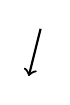
\begin{tikzpicture}[x=1cm,y=1cm]\draw[->,thick](.15,.6)--(0,0);\end{tikzpicture}}
\inserted{\[
\begin{aligned}
\operatorname{Hom}(K,\overline\sigma(X))&\simeq\operatorname{Hom}(\overline\sigma'K,X)\\
&\simeq\varprojlim_\lambda\varinjlim_\mu\operatorname{Hom}(K_\lambda,\sigma(X_\mu))\\
&\simeq\varprojlim_\lambda\varinjlim_\mu\operatorname{Hom}(\sigma'K_\lambda,\deleted{\unsure{\alpha}}X_\mu)
\end{aligned}
\]}

\diagram{\begin{tikzcd}[ampersand replacement=\&]
(\mathrm{Cons})\arrow[r,"{\text{pl. fid}}"]\&\underrightarrow{\operatorname{Hom}}((\mathrm{Cons\ cpt})^\circ,(\unsure{\mathrm{Cons}|\mathrm{Ens}}))
\end{tikzcd}}
\margin{119}

\scanpage{121}
\begin{center}- 93 -\end{center}
\margin{n\textsuperscript{o} 371}

$\bigwedge(N)$, où $N$ est un sous-module de type fini de $M$; il suffit alors d'appliquer le cor.3 de la prop.2 du n\textsuperscript{o} 1.

COROLLAIRE 5.- \uline{Soient} $N$, $P$ \uline{deux sous-modules d'un} $A$-\uline{module} $M$ \uline{tels que} $N\cap P$ \uline{soit facteur direct de} $N$ \uline{et de} $P$ \uline{et} $N+P$ \uline{facteur direct de} $M$. \uline{Alors} $\bigwedge(N)$ \uline{et} $\bigwedge(P)$ \uline{s'identifient canoniquement à des sous-algèbres de} $\bigwedge(M)$, \uline{et} $\bigwedge(N\cap P)$ \uline{à l'intersection} $\bigwedge(N)\cap\bigwedge(P)$.

En effet, si $E$, $F$ sont des supplémentaires de $N\cap P$ dans $N$ et $P$ respectivement et $G$ un supplémentaire de $N+P$ dans $M$, $M$ est somme directe des quatre sous-modules $N\cap P$, $E$, $F$, $G$; donc $\bigwedge(N)$, $\bigwedge(P)$ et $\bigwedge(N\cap P)$ s'identifient à des sous-algèbres de $\bigwedge(M)$ (cor.3). En outre, en vertu du cor.1, $\mathop{\bigwedge}\limits^n N$ (resp. $\mathop{\bigwedge}\limits^n P$) s'identifie à la somme directe des sous-modules $\mathop{\bigwedge}\limits^p(N\cap P)\otimes\mathop{\bigwedge}\limits^{n-p}E$ (resp. $\mathop{\bigwedge}\limits^p(N\cap P)\otimes\mathop{\bigwedge}\limits^{n-p}F$) pour $0\leq p\leq n$; on a donc bien $\bigwedge(N\cap P)=\bigwedge(N)\cap\bigwedge(P)$.

PROPOSITION 8.- \uline{Soit} $(e_\lambda)_{\lambda\in L}$ \uline{une base d'un} $A$-\uline{module} $M$; \uline{munissons} $L$ \uline{d'une structure d'ordre total}, \uline{et pour toute partie finie} $H$ \uline{de} $L$, \uline{posons}
\[
\text{(11)}\qquad e_H=e_{\lambda_1}\wedge e_{\lambda_2}\wedge\cdots\wedge e_{\lambda_n}
\]
\uline{si} $(\lambda_i)_{1\leq i\leq n}$ \uline{est la suite strictement croissante des éléments de} $H$. \uline{Alors les éléments homogènes} $e_H$, \uline{où} $H$ \uline{parcourt l'ensemble} $\unsure{\mathfrak F|\mathrm F}(L)$ \uline{des parties finies de} $L$, \uline{forment une base de} $\bigwedge(M)$.

Supposons d'abord $L$ \uline{fini}, soit par exemple $L=[\![1,m]\!]$ muni de l'ordre usuel; alors la proposition résulte de la prop.7, car si on pose $M_i=Ae_i$ pour $1\leq i\leq m$, $M$ est somme directe des $M_i$ et il résulte aussitôt du cor.3 de la prop.2 du n\textsuperscript{o} 1 que $\bigwedge(M_i)=A\oplus M_i$ (autrement dit $\mathop{\bigwedge}\limits^p M_i=0$ pour $p\geq2$); la conclusion résulte alors du cor.1 de la prop.7 et du chap.II, 3e éd., § 3, n\textsuperscript{o} 4, prop.4.

Supposons ensuite $L$ infini et pour toute partie finie $J$ de $L$, soit $M_J$ le sous-module de $M$ ayant pour base les $e_\lambda$ tels que $\lambda\in J$; il est clair que $M$ est limite
\margin{120}

\scanpage{122}
$X$ Schéma \unsure{compact}, [i.e. \unsure{quasi-compact} et \inserted{\uline{\unsure{topologiquement}}} \uuline{séparé}]

(i) $X$ est tot. discontinu, \deleted{i.e. si $x,y\in X$, $x\ne y$, alors il existe une \unsure{partie ouverte et fermée} de $X$ qui contient $x$ et non $y$. En effet, \unsure{soient} $U,V$ des ouverts, $U\ni x$, $V\ni y$, $U\cap V=\varnothing$.}
i.e. tt $x\in X$ a un syst. fond. de voisinages qui sont à la fois \uline{ouverts} et \uline{fermés}.

[En effet, il y a un syst. fond. de voisinages ouverts quasi-compacts]

(ii) $X$ \unsure{est} affine. En effet, \deleted{\unsure{prenons} \illegible{6} \illegible{3} \unsure{affines} \illegible{5}} \inserted{on recouvre $X$ par des ouverts affines en \unsure{n\textsuperscript{bre}} fini, soit $X_i$ $(1\leq i\leq n)$}. \deleted{\unsure{les}.} Ils sont ouverts \unsure{et} fermés. Soit
\[
X'_i=X_i-X_i\cap\bigcup_{j<i}X_j,
\]
Alors $X'_i$ est une partie ouverte et fermée de $X_i$, donc affine puisque $X_i$ l'est (\unsure{en vertu} p.ex. du \unsure{critère élém. pour} \unsure{immersions} \unsure{fermés|fermées}). Donc $X$ est \deleted{\unsure{et}} somme des $X'_i$, il est affine.

(iii) Les parties constructibles de $X$ sont des parties ouvertes et fermées. [\deleted{Donc} \inserted{\unsure{En eff.}} car $\mathrm{Cons}\,X\to X$ est un \deleted{\unsure{homéomorphisme}} \unsure{hom|bon}] Donc
\margin{121}

\scanpage{123}
\begin{center}- 92 -\end{center}
\margin{n\textsuperscript{o} 371}

\uline{de sous-modules}; \uline{pour tout} $i$, \uline{soit} $u_i=M_i\to N_i$ \uline{une application} $A$-\uline{linéaire et soit} $u=\bigoplus_{1\leq i\leq n}u_i:M\to N$. \uline{Alors le diagramme}
\diagram{\begin{tikzcd}[ampersand replacement=\&,column sep=large,row sep=large]
{}^{\mathrm g}\!\displaystyle\bigotimes_{1\leq i\leq n}(\bigwedge(M_i)) \arrow[r] \arrow[d,"{}^{\mathrm g}\!\bigotimes_{1\leq i\leq n}(\bigwedge(u_i))"'] \& \bigwedge(M) \arrow[d,"\bigwedge(u)"] \\
{}^{\mathrm g}\!\displaystyle\bigotimes_{1\leq i\leq n}(\bigwedge(N_i)) \arrow[r] \& \bigwedge(N)
\end{tikzcd}}
(\uline{où les flèches horizontales sont les isomorphismes définis dans la prop.7}) \uline{est commutatif}.

Il suffit de voir que les deux applications ${}^{\mathrm g}\!\bigotimes_i(\bigwedge(M_i))\to\bigwedge(N)$ définies par le diagramme prennent la même valeur dans chacun des modules $\bigotimes_{1\leq i\leq n}(\mathop{\bigwedge}\limits^{m_i}M_i)$, ce qui résulte aussitôt des définitions.

COROLLAIRE 3.- \uline{Soit} $u:M\to N$ \uline{une application} $A$-\uline{linéaire injective}, \uline{telle que} $u(M)$ \uline{soit facteur direct de} $N$. \uline{Alors l'homomorphisme} $\bigwedge(u):\bigwedge(M)\to\bigwedge(N)$ \uline{est injectif et} $\bigwedge(N)$ \uline{est somme directe de la sous-algèbre graduée} $\bigwedge(u)(\bigwedge(M))$ \uline{et d'un idéal bilatère gradué engendré par un supplémentaire de} $u(M)$ \uline{dans} $N$.

Cela résulte du cor.1 appliqué pour $n=2$, car la somme des sous-modules $(\mathop{\bigwedge}\limits^p M_1)\otimes(\mathop{\bigwedge}\limits^q M_2)$ pour tous les couples $(p,q)$ tels que $p\geq1$ n'est autre que l'idéal bilatère $m_1\otimes(\bigwedge(M_2))$ de $(\bigwedge(M_1))\otimes^{\mathrm g}(\bigwedge(M_2))$, où $m_1$ est la somme directe des $\bigwedge(M_1)$ pour $p\geq1$, idéal bilatère de $\bigwedge(M_1)$. On peut aussi donner une démonstration directe n'utilisant pas la prop.7 et calquée sur celle du § 4, n\textsuperscript{o} 2, prop.4.

COROLLAIRE 4.- \uline{Tout élément} $z$ \uline{de} $\bigwedge(M)$ \uline{dont la composante homogène scalaire} (i.e. \uline{de degré} 0) \uline{est nulle}, \uline{est nilpotent}.

Il est clair en effet que tout élément de $\bigwedge(M)$ appartient à une sous-algèbre
\margin{122}

\scanpage{124}
\begin{flushright}\uline{Greenberg} - \uline{Néron}\end{flushright}
\margin{123}

\scanpage{126}
Soit $\deleted{\unsure{\mathcal X}=}(X_i)_{i\in I}$ un système projectif de préschémas, essentiellement affine [i.e. $\exists i_0$, $\forall i\geq i_0$, $\varphi_{i_0i}$ est affine]. Alors $X=\varprojlim_i X_i$ existe, $\mathrm{Top}\,X=\varprojlim_i\mathrm{Top}(X_i)$ $\ldots$.

Soit $x\in X$, on dit que $\unsure{X|x}$ est \uline{épais} si

(Ép) $\exists i$ t.q. $\forall j\geq i$, $x_j$ est un p\textsuperscript{t} maximal de $\varphi_{ij}^{-1}(x_i)$, donc si $k\geq j\geq i$, $\deleted{\unsure{\varphi}}x_k$ est maximal de $\varphi_{jk}^{-1}(x_j)$.

\unsure{Sous quelles conditions est équivalent|Sous quelles conditions est épaisseur}:

(Ép)$'$ $\exists i$, \deleted{t.q.} et une partie ouverte non vide $U_i$ de $\bar x_i$, t.q. $\forall j\geq i$, $\varphi_{ij}^{-1}(U_i)\subset\bar x_j$ (Alors la même propriété est vraie pour $\forall i'\geq i$).

Cela \unsure{prouve} que $\varphi_{ij}^{-1}(U_i)$ est irréductible, de p\textsuperscript{t} générique $x_j$, et donc (Ép)$'$ implique (Ép)\unsure{?}.

Considérons aussi

(Ép)$''$ $\bar x$ \inserted{$=\varprojlim\bar x_i$} est une partie \uline{constructible} de $X$.

Ceci équivaut \inserted{(si $X_i$ sont \unsure{noeths})} à: $\bar x=\varphi_i^{-1}(\bar x_i)$ pour $i$ \unsure{grandement|grand assez} \deleted{(car: pour $i$ \unsure{constructible} $\ldots$)} (donc pour $i'\geq i$)

(Ép)$'''$ $\exists$ une partie constructible \deleted{\unsure{non fermée}} \inserted{ouverte non vide} de $\bar x$, soit $U$.

i.e. $\exists U_i$
\margin{125}

\scanpage{127}
\begin{center}- 145 -\end{center}
\margin{n\textsuperscript{o} 316}

Si $x\longrightarrow x_M$ est une représentation irréductible de dimension finie, si $\beta$ est la forme bilinéaire associée, et si $\dim\unsure{h|\mathfrak h}$ n'est pas divisible par la caractéristique de $K$, montrer que $H^p(\unsure{g|\mathfrak g},M)=\{0\}$ pour tout $p$. (Utilisant la prop.12, montrer que $\unsure{\mathbf T|\mathrm T}$ est un automorphisme de $C^*(\unsure{g|\mathfrak g},M)$, donc induit des automorphismes de $Z^p(\unsure{g|\mathfrak g},M)$ et $B^p(\unsure{g|\mathfrak g},M)$. Pour $f\in Z^p(\unsure{g|\mathfrak g},M)$, $\begin{aligned}\unsure{\mathbf T|\mathrm T}f&=\\&=(d\rho+\rho d)f=d\rho f\in B^p(\unsure{g|\mathfrak g},M)\end{aligned}$, d'où $Z^p(\unsure{g|\mathfrak g},M)=B^p(\unsure{g|\mathfrak g},M)$).
\figure{\begin{tikzpicture}\draw[line width=.6pt] (0,0)--(2.5,0);\end{tikzpicture}}
\margin{126}

\scanpage{128}
$x$ maximal dans $\varphi_i^{-1}(\unsure{x_i})$

\diagram{\begin{tikzcd}[ampersand replacement=\&,column sep=small,row sep=small,execute at end picture={\draw[rounded corners] ([xshift=-8pt,yshift=8pt]\tikzcdmatrixname-1-2.north west) rectangle ([xshift=5pt,yshift=-8pt]\tikzcdmatrixname-2-4.south east);}]
\& (\text{Ép})' \arrow[r,Rightarrow] \arrow[dr,Rightarrow] \& (\text{Ép})+(\uline{\unsure{\text{unicité : fibre de }x_i}}) \& \\
\& \deleted{(\text{Ép})'''} \& (\text{Ép})''' \arrow[r,Rightarrow] \& \begin{gathered}\text{si }\deleted{\unsure{\forall x'_i}}X'_i,\ \exists\text{ un ouvert }\ne\varnothing\\ U_i\subset\bar x_i\text{ t.q. les }\varphi_{ij}^{-1}(U_i)\unsure{\times|\cap}X'_j=\varphi_j(X)\end{gathered}\quad ??? \\
(\text{Ép})'' \arrow[uur,Rightarrow,"\substack{\text{M.L.}\\\text{et }I=\mathbf N}"] \arrow[urr,Rightarrow,"4"'] \& \& \&
\end{tikzcd}}

\margin{$\deleted{\unsure{E}}\quad\text{p\textsuperscript{t} épais}\longleftarrow\substack{\text{\unsure{fermés} constructibles}\\\text{irréductibles}}$}

\[
U_j\cap X'_j\subset\bar x_j\qquad X'_i\longleftarrow X'_j
\]
\[
U_i\subset\bar x_i
\]
\margin{$x\in E\subset\bar x$}
\margin{$x\in U_0\cap Z_0$}
\margin{$\bar x$}

\[
x\in\deleted{\unsure{\bar x}}\bigcup_i U_i\cap Z_i
\]
\diagram{\begin{tikzcd}[ampersand replacement=\&,column sep=small,row sep=large]
\unsure{\mathcal X|\mathfrak X} \arrow[dr] \& \& \unsure{\mathcal X_i|\mathfrak X_i} \arrow[dl] \\
\& {} \&
\end{tikzcd}}

\[
x\in U_0\cap Z_0\subset\bar x
\]
\[
\deleted{\bar x\unsure{\in}\ \unsure{x_0}\in Z_0}\qquad
\bar x=\overline{U_0}\cap Z_0\subset Z_0
\]
$\unsure{U_0}$

$f_1\quad f_n$ \unsure{nuls en} $x$
\[
f_1\cdots f_n\in p\qquad g
\]
\[
\text{si }g\notin q\qquad q\supset p\Longleftrightarrow q\supset f_1\cdots f_n
\]
\figure{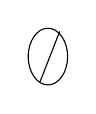
\begin{tikzpicture}\draw (0,0) ellipse (.25 and .36);\draw (-.1,-.32)--(.15,.32);\end{tikzpicture}}
\[
\mathcal O_{X,x}\qquad \unsure{\mathfrak m|m}_x\quad\deleted{\text{\unsure{idéal}}}
\]
$A_g$: un \unsure{idéal de définition}

\margin{\unsure{idéal de} \deleted{\unsure{type}} \unsure{un} \unsure{type fini} \unsure{d'où}}
\margin{127}

\scanpage{129}
\begin{center}- 135 -\end{center}
\margin{n\textsuperscript{o} 316}

a) L'algèbre $\widetilde U$ et l'application $\widetilde{\unsure{\varrho|\rho}}$ sont solutions d'un problème d'application universelle: pour tout p-homomorphisme $f$ de $\unsure{g|\mathfrak g}$ dans une algèbre associative $B$ sur $K$ (considérée comme p-algèbre de Lie), il existe un K-homomorphisme et un seul $f'$ de $\widetilde U$ dans $B$ (pour les structures d'algèbres associatives) tel que $f=f'\circ\widetilde{\unsure{\varrho|\rho}}$.

b) Montrer que si $(b_\lambda)_{\lambda\in\Lambda}$ est une base de $\unsure{g|\mathfrak g}$ ($\Lambda$ étant totalement ordonné), $\widetilde{\unsure{\varrho|\rho}}$ est injective, et que, si on identifie $x$ et $\widetilde{\unsure{\varrho|\rho}}(x)$ pour $x\in\unsure{g|\mathfrak g}$, les éléments $\prod_\lambda b_\lambda^{\nu_\lambda}$ (où les $\lambda$ vont en croissant, où les $\nu_\lambda$ sont nuls sauf un nombre fini d'entre eux, et où $0\leq\nu_\lambda<p$ pour tout $\lambda$) forment une base de $\widetilde U$. (Identifiant canoniquement $\unsure{g|\mathfrak g}$ à un sous-module de $U$, on pose $\varphi(x)=x^p-x^{[p]}$ pour tout $x\in\unsure{g|\mathfrak g}$. Pour tout indice composé $\alpha=(\alpha_\lambda)\in\mathbf N^{(L)}$, soit $\alpha_\lambda=\beta_\lambda+p\gamma_\lambda$ avec $0\leq\beta_\lambda<p$, et soit $T_\alpha=(\prod_\lambda b_\lambda^{\beta_\lambda})(\prod_\lambda(\varphi(b_\lambda))^{\gamma_\lambda})$. Montrer que les $T_\alpha$ forment une base de $U$ et les $T_\alpha$ tels que $\gamma=(\gamma_\lambda)\ne0$ une base de $J$; on observera que les $\varphi(b_\lambda)$ appartiennent au centre de $U$).

7) - Soit $\unsure{g|\mathfrak g}$ une p-algèbre de Lie sur un anneau $K$ de caractéristique $p>0$ ($p$ premier). On dit qu'une dérivation $D$ de $\unsure{g|\mathfrak g}$ est une \uline{p-dérivation} si on a $D(x^p)=(\mathrm{ad}\,x)^{p-1}.dx$ pour tout $x\in\unsure{g|\mathfrak g}$. Toute dérivation intérieure est une p-dérivation.

a) Si $L$ est une K-algèbre associative, toute dérivation de $L$ est une p-dérivation lorsque $L$ est considérée comme p-algèbre de Lie. (Utiliser la formule (2) de l'exerc. 19 du § 1).

b) Supposons que $\unsure{g|\mathfrak g}$ ait une base. Pour qu'une dérivation de $\unsure{g|\mathfrak g}$ soit une p-dérivation, il faut et il suffit qu'elle puisse se prolonger en une dérivation de l'algèbre enveloppante restreinte de $\unsure{g|\mathfrak g}$.
\margin{128}

\scanpage{131}
$V$ anneau de valuation discrète, corps résiduel $k$ parfait, corps des fractions $K$.

Pour tout préschéma $X$ sur $V$, on définit $\bar X$ par Greenberg.
\[
\bar X(k')\simeq X(V_{k'})\deleted{\unsure{\longrightarrow}X}
\]
\margin{($k'$ \unsure{alg.} sur $k$, $V_{k'}$ \unsure{ext. correspondante de} $V$)}

Si $k'$ est parfait, $V_{k'}$ est un anneau de valuation discrète, soit $K_{k'}=K'$ son corps des fractions, on a
\[
\bar X(\unsure{k|k'})\simeq X(V_{k'})\longrightarrow X(K')
\]

Soit $\deleted{\unsure{\varphi:X\longrightarrow}}Y$ un autre $V$ préschéma, \inserted{\uline{propre sur} $V$,} et soit
\[
\varphi:X_K\longrightarrow Y_K
\]
un morphisme de $K$-préschémas, nous allons en déduire une \uline{application ensembliste}
\[
\bar\varphi:\bar X\longrightarrow\bar Y.
\]

Soit en effet $\bar x\in\bar X$, soit $k'=\widetilde{k}(\bar x)$ \deleted{une} \inserted{``la''} clôture parfaite de $k(\bar x)$, alors $\bar x$ définit un p\textsuperscript{t} $\bar x'\in\bar X(k')$, d'où un p\textsuperscript{t} \deleted{\unsure{générique}} $\alpha_X(\bar x')\in\bar X(V_{k'})\subset\bar X(K_{k'})$ et appliquant un point
\[
\varphi(\alpha_X(\bar x'))\in\overset{\deleted{\rule{.6em}{.3pt}}}{Y}(K_{k'})
\xleftarrow{\sim}\overset{\deleted{\rule{.6em}{.3pt}}}{Y}(V_{k'})
\xleftarrow[\sim]{\alpha_Y}\bar Y(k'),
\]
dont la \unsure{localité} est notée $\bar\varphi(x)$. On a donc par construction un homo
\[
k(\varphi(\bar x))\longrightarrow\widetilde{k(\bar x)}
\]
(ici le $\sim$ dénote la clôture parfaite).

\margin{Si $\overset{\deleted{\rule{.6em}{.3pt}}}{Y}$ n'est pas propre sur $V$ et $\varphi$ seulement \unsure{application rationnelle}, on aura une ``application \unsure{non} \unsure{partout définie}'' $\bar X\longrightarrow\bar Y$, ayant les propriétés}

Par la suite, $X,Y$ de type fini sur $K$, et \inserted{\unsure{géom.}} intègres

\uline{Proposition 1} Supposons $\bar x\in\bar X$ \uline{épais} et $\varphi$ \uline{dominant gén.\textsuperscript{t} séparable} [i.e. fibre gén. séparable]. Alors \inserted{\unsure{si|1\textsuperscript{o}}} $\bar y=\varphi(\bar x)$ \inserted{\unsure{existe, et|étale, et}} est \uline{épais}, $k(\bar y)\subset k(\bar x)$, et l'application ponctuelle $\bar x_{\mathrm{red}}\longrightarrow\bar y_{\mathrm{red}}$ définie par cette inclusion provient d'un \unsure{promorphisme} d'indice fini sur un ouvert constructible dense $U\in\bar x$, [d'image un ouvert constructible de $\bar y_{\mathrm{red}}$].
\figure{\begin{tikzpicture}\draw (0,0)--(0,-2);\end{tikzpicture}}
\margin{130}

\scanpage{132}
\uline{Corollaire} Fonctorialité \figure{\begin{tikzpicture}\node[draw,ellipse,inner sep=5pt] {en $X_K$};\end{tikzpicture}} de l'ensemble $\mathrm{Ép}\deleted{\unsure{\mathrm{ais}}}(\bar X)$ des points \deleted{\unsure{de}} épais de $\bar X$ [\unsure{munis} de leurs corps résiduels $\ldots$], pour des \deleted{morphismes} \inserted{applic. rationnelles} $X_K-Y_K$ \uline{dominantes gén.\textsuperscript{t} séparables de} $K$-\uline{schémas} \uline{propres}.

\uline{Proposition 2} Soit $S$ une partie constructible de $\bar X$, $X_K$-simple, [tel que $\unsure{\ell|d}(\unsure{W|V},x)$ y soit borné], et tel que $\bar\varphi(S)$ existe [p.ex $Y$ propre sur $V$] et soit $Y_K$-simple.

Alors $\bar\varphi(S)$ est constructible. De plus, il y a une partition \inserted{finie} $S=\coprod_i S_i$, les $S_i$ des sous-schémas irréductibles constructibles de $X$, telle que $\varphi$ soit morphique d'indice fini sur chaque $S_i$, [et $\varphi(S_i)$ est alors un ens. constructible irréductible $\ldots$]

\uline{Corollaire} Fonctorialité en $X_K$ variant comme dessus, et de plus simple sur $K$, de l'ens. $\mathrm{Cons}(\bar X)$ des parties constructibles de $\bar X$.
\margin{131}

\scanpage{134}
Considérons le foncteur d'anneaux [ou de préschémas \uline{quasi-compacts}]
\[
\Gamma:A\longmapsto A((t))^*=(A[[t]]_t)^*
\]
\margin{($t$ une indéterminée)}

Ce foncteur est ind-représentable par un
\[
\mathcal G=\varinjlim_n(\mathcal G_n)
\]
\margin{$\varinjlim$ par abus de langage \unsure{ici!}}
$\mathcal G_n$ représente le sous-foncteur $\Gamma_n$ de $\Gamma$, où une série formelle $\deleted{A\longmapsto A((t))^*}\sum_{-\infty}^{+\infty}a_i t^i$ \inserted{ayant l'inverse $\sum_{-\infty}^{+\infty}b_jt^j$} est dans $\Gamma_n$ si $a_i=0$, $b_i=0$ pour $\unsure{i<-n|i<n}$. $\mathcal G_n$ est affine et en fait un sous-schéma fermé de $\mathrm{Spec}\,\mathbf Z[(a_i,b_i)_{i\geq-n}]$, [défini par les \deleted{relations} idéal des relations exprimant
\[
\Bigl(\sum_i a_it^i\Bigr)\Bigl(\sum_j b_jt^j\Bigr)=1,
\]
savoir $a_{-n}b_{-n}=0,\ldots$,]

\deleted{En particulier,} \inserted{Soit} $\Gamma_0$ est le foncteur
\[
\Gamma_0:A\longmapsto A[[t]]^*
\]
qui est représenté par
\[
\mathcal G_0=\mathbf G_m\times\mathrm{Spec}\,\mathbf Z[(a_i)_{i\geq1}]
\]
considérons le schéma
\[
\mathcal G'=\mathbf Z_{\mathbf Z}\times\mathcal G_0
\]
qui représente un foncteur ind-représentable
\[
\unsure{\mathcal G'|\Gamma'}=\underset{n}{\underset{\unsure{-|\rightarrow}}{\lim}}\unsure{\mathcal G'_n|\Gamma'_n}
\]
\[
\mathcal G'_n=[\unsure{-n|n},n]_{\mathbf Z}\times\mathcal G_0.
\]
On a un morphisme canonique
\[
\mathcal G'\longrightarrow\mathcal G
\]
\margin{133}

\scanpage{135}
correspondant à des morphismes
\[
\mathcal G'_n\longrightarrow\mathcal G_n
\]
\deleted{\unsure{et|de} \unsure{à} \unsure{l'homo} de \unsure{foncteurs}}
ou encore, composante par composante, à
\[
\varphi_n^\nu:\mathcal G_0\longrightarrow\mathcal G_n\qquad \nu\in[-n,+n]
\]
donné \deleted{par} sur les foncteurs par
\[
\varphi_n^\nu\left(\sum_{i\geq0}a_it^i\right)=t^\nu\sum a_it^i
\]

Ceci posé, on a un

\uline{Th} (i) Le morph. $\unsure{f_n|h_n}:\mathcal G'_n-\mathcal G_n$ est une \uline{immersion fermée surjective}\figure{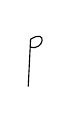
\begin{tikzpicture}[baseline]\draw (0,0)--(.03,.6)..controls(.25,.74)and(.2,.45)..(.03,.5);\end{tikzpicture}}. (ii) Elle induit une immersion ouverte sur $\mathcal G_0\times\{\nu\}$ pour $\nu=\pm n$, mais pour $-n<\nu<+n$, le morphisme induit \uline{n'est pas} une immersion ouverte [même après changement de base quelconque $S\longrightarrow\mathrm{Spec}\,\mathbf Z$, $S\ne\varnothing$]. (iii) Soit $\mathcal G_n^i$ le sous schéma ouvert \inserted{induit} et fermé de $\mathcal G_n$ \deleted{\unsure{image}} par l'image ensembliste $\deleted{\unsure{\varphi_n^i}}\varphi_n(\mathcal G_0\times\{i\})$, où $|i|\leq n$.

\margin{\figure{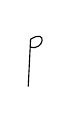
\begin{tikzpicture}[baseline]\draw (0,0)--(.03,.6)..controls(.25,.74)and(.2,.45)..(.03,.5);\end{tikzpicture}} donc $\mathcal G_n$ est réunion disjointe d'ouverts $\mathcal G_n^i$ $(i\in[-n,+n])$, d'ailleurs irréductibles, qui sont les images des $\varphi_n^i$}

Pour $n$ variable, on trouve ainsi un système ``inductif'' \inserted{d'immersions} de préschémas, ayant \unsure{même} \deleted{\unsure{type foncteur}} top. sous-jacent. Donc \unsure{si} $n'\geq n\geq|i|$, le morphisme $\mathcal G_n^i\longrightarrow\mathcal G_{n'}^i$ n'est pas un isomorphisme, et ceci même sur une base $S\ne\varnothing$ quelc.

[Il suffit de regarder sur les corps premiers $\ldots$].
\margin{134}

\scanpage{136}
\diagram{\begin{tikzcd}[ampersand replacement=\&,column sep=large,row sep=large]
 \& \mathrm{Pro}(\mathrm{Sch}/S) \arrow[d,phantom,"\cup"{description},"{\substack{\text{sous-catégorie}\\\text{pleine}}}"{anchor=west,xshift=8pt}] \& \text{pro-préschémas}\\
(\mathrm{Sch}/S) \& \mathrm{Pro}'(\mathrm{Sch}/S) \arrow[l,"\varprojlim"'] \arrow[d,phantom,"\cup"{description},"{\substack{\text{sous-catégorie}\\\text{pleine}}}"{anchor=west,xshift=8pt}] \& \text{pro-préschémas }(X_i)_{i\in I},\ \text{t.q. }\exists i,\ \unsure{u_{ji}|\varphi_{ij}}\ \text{affines pour }j\geq i\\
 \& \mathrm{Pro}''(\mathrm{Sch}/S) \arrow[ul,"{\substack{\text{foncteur}\\\text{pleinement}\\\text{fidèle}}}"{anchor=north east,xshift=-5pt,yshift=-3pt}] \& \text{pro-préschémas }(X_i)_{i\in I}\ \text{t.q.}
\end{tikzcd}}
\deleted{\[\left\{\begin{array}{l}\unsure{X_i\ \text{quasi-cpt. et de présentation finie}}\\ \exists i,\ [\unsure{u_{ji}|\varphi_{ij}}\ \text{affines de prés. }\unsure{\text{finie}}]\end{array}\right.\]}
\[
\left\{\begin{array}{l}
\forall i\,\unsure{\mathrm{gd}|\mathrm{quel}},\ X_i\ \text{est qu. cpt et de présentation finie sur }S\\
\exists i\ \text{t.q. }j\geq i\ \text{implique }\unsure{u_{ji}|\varphi_{ij}}\ \text{affine.}
\end{array}\right.
\]

Soient $\unsure{\mathcal X|\mathfrak X}\in\mathrm{Ob}\,\mathrm{Pro}''(\mathrm{Sch}/S)$, $\mathcal Y\in\mathrm{Ob}\,\mathrm{Pro}'(\mathrm{Sch}/S)$ \inserted{$\mathcal Y=(Y_j)$, les $Y_j$ quasicompacts}, alors
\[
\mathrm{Hom}_{\mathrm{Pro}(\mathrm{Sch}/S)}(\mathcal Y,\unsure{\mathcal X|\mathfrak X})\overset{\sim}{\longrightarrow}\mathrm{Hom}(\varprojlim\mathcal Y,\varprojlim\unsure{\mathcal X|\mathfrak X})
\]
\deleted{[En particulier, la catégorie}
\inserted{Si on est sur une base $S$}
\[
\mathrm{Hom}_{\mathrm{Pro}(\mathrm{Sch}/S)}(\mathcal Y,\unsure{\mathcal X|\mathfrak X})\overset{\sim}{\longrightarrow}\mathrm{Hom}_S(\varprojlim\mathcal Y,\varprojlim\unsure{\mathcal X|\mathfrak X})
\]

\deleted{Dans les provariétés de Serre}

\uline{Remarque} Dans Serre et Néron, on utilise des systèmes projectifs de schémas \inserted{(algébriques)} qui sont \inserted{(pratiquement tjs)} $\in\mathrm{Pro}''(\mathrm{Sch})$.
\deleted{\unsure{Donc}} Il y a avantage à les ``interpréter'' comme étant de véritables schémas sur $k$, \unsure{et non bien|et non rien} des pro-objets $\ldots\ldots$.
\figure{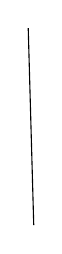
\begin{tikzpicture}\draw (0,0)--(-.07,2.5);\end{tikzpicture}}
\margin{135}

\scanpage{138}
\mspage{1}
\deleted{$a_{i0}$}
\[
\left\{\begin{array}{l}
f_i=a_i+\displaystyle\sum_{1\leq j\leq n}b_{ij}t_j+\displaystyle\sum_{|p|\geq2}c_{ip}t^p\\[-2pt]
\hspace{2em}\deleted{\unsure{\in\mathfrak m|0}}\\
1\leq i\leq n
\end{array}\right.
\qquad a_i,b_{ij},c_{ip}\in A
\qquad\left\{\begin{array}{l}a_i\in\mathfrak m\\ \det(b_{ij})\unsure{\notin|\in}\unsure{A\mathfrak m|A^\times}\end{array}\right.
\]
\diagram{\begin{tikzcd}[ampersand replacement=\&,column sep=huge]
(\lambda_1,\unsure{-|\ldots}\lambda_n)\in\mathfrak m^{(\times n)} \arrow[r,squiggly,"\lambda_{(f=(f_1,\unsure{-|\ldots} f_n))}"'] \& (f_1(\lambda_1,\unsure{-|\ldots},\lambda_n),\unsure{-|\ldots},f_n(\lambda_1,\unsure{-|\ldots}\lambda_n))
\end{tikzcd}}

Si $A$ est d'ordre infinitésimal $N$, alors $\lambda_f$ est connu quand on connaît $f\mod(t_1,\unsure{-|\ldots} t_n)^{N+1}$, donc \unsure{quand on} connaît \deleted{les} $\unsure{N|n}$ \uline{polynômes} en $t$ de degré $\leq N$.
\deleted{\unsure{ou}}
\[
\boxed{f_i(\lambda_1,\unsure{-|\ldots}\lambda_n)=a_i+\sum_jb_{ij}\lambda_j+\sum_{2\leq|p|\leq N}c_{ip}\lambda_1^{p_1}\unsure{-|\ldots}\lambda_n^{p_n}}
\]
\diagram{\begin{tikzcd}[ampersand replacement=\&]
B=A[[t_1,\unsure{-|\ldots} t_n]]\\
A\arrow[u]
\end{tikzcd}}
\figure{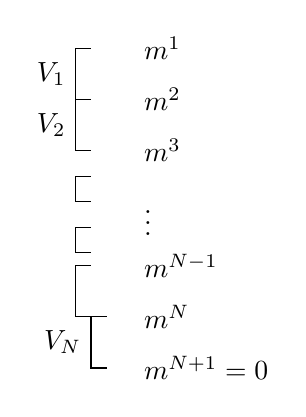
\begin{tikzpicture}[x=1cm,y=.65cm]
\node[anchor=west] at (1,0) {$\mathfrak m^{\deleted{\unsure{1}}}$};
\node[anchor=west] at (1,-1) {$\mathfrak m^2$};
\node[anchor=west] at (1,-2) {$\mathfrak m^3$};
\node[anchor=west] at (1,-3.25) {$\vdots$};
\node[anchor=west] at (1,-4.25) {$\mathfrak m^{N-1}$};
\node[anchor=west] at (1,-5.25) {$\mathfrak m^N$};
\node[anchor=west] at (1,-6.25) {$\mathfrak m^{N+1}=0$};
\draw (.45,0)--(.25,0)--(.25,-1)--(.45,-1);
\draw (.45,-1)--(.25,-1)--(.25,-2)--(.45,-2);
\draw (.45,-2.5)--(.25,-2.5)--(.25,-3)--(.45,-3);
\draw (.45,-3.5)--(.25,-3.5)--(.25,-4)--(.45,-4);
\draw (.45,-4.25)--(.25,-4.25)--(.25,-5.25)--(.45,-5.25);
\draw (.65,-5.25)--(.45,-5.25)--(.45,-6.25)--(.65,-6.25);
\node[left] at (.25,-.5) {$V_1$};\node[left] at (.25,-1.5) {$V_2$};\node[left] at (.45,-5.75) {$V_N$};
\end{tikzpicture}}
\margin{137}

\scanpage{139}
\begin{center}- 132 -\end{center}
\margin{n\textsuperscript{o} 316}

terme constant, et utiliser le fait que la sous-algèbre des $X\in\unsure{\mathrm{gl}|\mathfrak{gl}}(n,K)$ telles que ${}^tXR+RX=0$ est de dimension $n(n-1)/2$ ).

c) Définir de même le \uline{groupe symplectique formel} à $2n$ variables sur un corps (commutatif) $K$ quelconque, et montrer que son algèbre de Lie s'identifie à la sous-algèbre de $\unsure{\mathrm{gl}|\mathfrak{gl}}(2n,K)$ formée des matrices $X$ telles que ${}^tXA+AX=0$, où $A=\begin{pmatrix}0&I_n\\-I_n&0\end{pmatrix}$

27) - Soient $K$ un corps de caractéristique $p>0$, $G$ le groupe formel de dimension $2$ défini par $f_1(x,y)=X_1+Y_1+X_1Y_1$, $f_2(x,y)=X_2+Y_2(1+X_1^p)$. Montrer que $G$ n'est pas commutatif, mais que son algèbre de Lie est commutative.
\margin{138}

\scanpage{140}
\[
G_{n,N}=\uline{\mathrm{Aut}}_{\text{Algèbre augmentée}}\ \mathbf Z[t_1,\ldots,t_n]/(t_1,\ldots,t_n)^{N+1}
\]
$\Gamma_{n,\deleted{\unsure{N}}}=\mathrm{Grb}(G_{n,N})$ groupe algébrique sur $k$ des changements de coordonnées
\[
\left\{\begin{array}{l}
f_i(t_1,\unsure{-|\ldots}t_n)=\displaystyle\sum_jb_{ij}\unsure{t'_j|t_j}+\displaystyle\sum_{2\leq|p|\leq N}c_{ip}t_1^{p_1}\unsure{-|\ldots}t_n^{p_n}\\
b_{ij},c_{ip}\in A,\qquad\det(b_{ij})\notin\mathfrak m
\end{array}\right.
\]
Ce groupe opère sur $\mathfrak m^n$ si $A$ est d'ordre infinitésimal $\leq N$. \deleted{\unsure{Donc}}

\[
\begin{array}{ll}
f\in\Gamma_n & x\mapsto T_f(x)+a\\
a\in\mathfrak m^n & \\
&\deleted{T_g}\quad b+T_g(\deleted{\unsure{0}}a+T_f(x))\\[3pt]
&b+T_g(a)+
\end{array}
\]
\[
\begin{array}{ll}
\unsure{T_{g'}|T_g}(a+b)&g(x+y)=g(x)\\[5pt]
\deleted{\unsure{T}}\quad\deleted{\unsure{\xi}}\quad\unsure{g}(a+b)=g(a)+g'&\\[5pt]
g(x+y)=&
\end{array}
\]
\margin{139}

\scanpage{141}
\begin{center}- 129 -\end{center}
\margin{n\textsuperscript{o} 316}

où, dans la série $o_3$, tous les monômes sont de degré $\geq3$, par rapport à l'ensemble des $Y_i$ et des $Z_i$. En déduire que :
\[
\begin{aligned}
(3)\quad u(f(x,y))-u(f(y,x))&=\sum_{i<j}(X_iY_j-X_jY_i)([T_i,T_j]^{(e)}(u))+\\
&\quad+o'_3(x,y)
\end{aligned}
\]
où tous les termes de $o'_3$ sont de degré total $\geq3$. Montrer que si $G$ est commutatif, $\unsure{g|\mathfrak g}$ est commutative.

d) Soit $G'$ un second groupe formel, de dimension $n$, dont la loi de groupe est $f'$. On appelle \uline{homomorphisme formel} de $G$ dans $G'$ un système $F=(F_j(x))_{1\leq j\leq m}$ d'éléments de $A_x$ tel que l'on ait $f'(F(x),F(y))=F(f(x,y))$. Pour toute dérivation invariante à gauche $D\in\unsure{g|\mathfrak g}$, montrer que $v\longrightarrow D(v\circ F)$ est une dérivation invariante à gauche appartenant à l'algèbre de Lie $\unsure{g'|\mathfrak g'}$ de $G'$. Si on la désigne par $F^*(D)$, $F^*$ est un homomorphisme (un p-homomorphisme pour $p>0$) de $\unsure{g|\mathfrak g}$ dans $\unsure{g'|\mathfrak g'}$. Si $(T_i)_{1\leq i\leq n}$, $(T'_j)_{1\leq j\leq m}$ sont les bases de $\unsure{g|\mathfrak g}$ et $\unsure{g'|\mathfrak g'}$ telles que $T_i^{(e)}=D_i^{(e)}$ et ${T'_j}^{(e)}={D'_j}^{(e)}$, montrer que la matrice de $F^*$, rapportée à ces bases, est la matrice $(\partial F_j/\partial X_i)_c$ (terme constant de $\partial F_j/\partial X_i$, où $i$ est l'indice des lignes, $j$ celui des colonnes).

25) - On appelle \uline{groupe linéaire formel} à $n$ variables sur le corps $K$, et on désigne par $\mathrm{GL}(n,K)$ (lorsqu'aucune confusion n'est possible) le groupe formel de dimension $n^2$ dont la loi de groupe est définie par
\[
f_{ij}(u,v)=-\delta_{ij}+\sum_{k=1}^n(\delta_{ik}+U_{ik})(\delta_{kj}+V_{kj})
\]
($\delta_{ij}$ indice de Kronecker ; les $3n^2$ indéterminées de la définition générale de l'exerc. 24 sont ici notées $U_{ij}$, $V_{ij}$, $W_{ij}$ avec $2$ indices variant de $1$ à $n$). Montrer que, si $D_{ij}=\partial/\partial U_{ij}$, les dérivations
\margin{140}

\scanpage{142}
\deleted{$\mathfrak m/\mathfrak m^2$}
\[
\begin{array}{ll}
\text{\unsure{espace} affine sous}&\unsure{\mathcal T|\mathcal J}^{0}_{B_0/A_0}\otimes V_1\\
\text{\unsure{espace} affine sous}&\unsure{\mathcal T|\mathcal J}^{0}_{B_0/A_0}\otimes V_2\\
&\unsure{\mathcal T|\mathcal J}^{0}_{B_0/A_0}\otimes V_3\qquad\unsure{\mathcal T|\mathcal J}_{V_0/}
\end{array}
\]
\figure{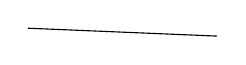
\begin{tikzpicture}\draw (0,0)--(2.4,-.1);\end{tikzpicture}}

$G_{A,n}=$ groupe algébrique sur $k$ des changements de \unsure{base} de la forme
\[
\left\{\begin{array}{l}
f_i=a_i+\displaystyle\sum_jb_{ij}t_j+\displaystyle\sum_{2\leq|p|\leq N}c_{ip}t^p\qquad a_i,b_{ij},c_{ip}\in A\\
a_i\in\mathfrak m,\ \det(b_{ij})\notin\mathfrak m
\end{array}\right.
\]

$G_n$ groupe sur $\mathbf Z$ des changements de \unsure{base}
\[
\left\{\begin{array}{l}
f_i=a_i+\displaystyle\sum\unsure{a_j|b_{ij}}t_j+\displaystyle\sum_{2\unsure{\leq|<}|p|\leq N}c_{ip}t_1^{p_1}\unsure{-|\ldots}t_n^{p_n}\\
\det(b_{ij})\ne0
\end{array}\right.
\]
i.e. les automorphismes de

\[
\deleted{\unsure{a+t}}\quad a_0+a_1t+a_2t^2
\]
\[
\deleted{a'_0+a'_1(a_0+a_1t)+\unsure{a'_2a_0^2}}
\]
\figure{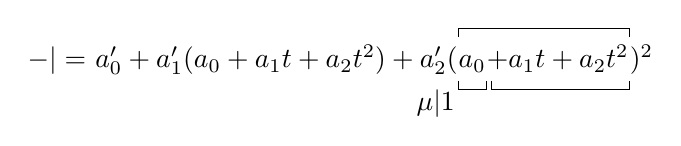
\begin{tikzpicture}[baseline=(prefix.base),inner sep=0pt]
\node[anchor=base west] (prefix) at (0,0) {$\unsure{-|=}\ a'_0+a'_1(a_0+a_1t+a_2t^2)+a'_2($};
\node[anchor=base west] (constant) at (prefix.base east) {$a_0$};
\node[anchor=base west] (tail) at (constant.base east) {$+a_1t+a_2t^2$};
\node[anchor=base west] at (tail.base east) {$)^2$};
\coordinate (upperleft) at (constant.west |- tail.north);
\coordinate (lowerleft) at (constant.west |- tail.south);
\coordinate (lowermid) at (constant.east |- tail.south);
\draw ([yshift=3pt]upperleft)--([yshift=6pt]upperleft)--([yshift=6pt]tail.north east)--([yshift=3pt]tail.north east);
\draw ([yshift=-3pt]lowerleft)--([yshift=-6pt]lowerleft)--([yshift=-6pt]lowermid)--([yshift=-3pt]lowermid);
\draw ([xshift=2pt,yshift=-3pt]tail.south west)--([xshift=2pt,yshift=-6pt]tail.south west)--([yshift=-6pt]tail.south east)--([yshift=-3pt]tail.south east);
\node[anchor=north east] at ([xshift=-1pt,yshift=-6pt]lowerleft) {$\unsure{\mu|1}$};
\end{tikzpicture}}
\[
k[t]/(t^3)\qquad
\boxed{\begin{aligned}
={}&(a'_0+a'_1a_0+a'_2a_0^2)\\
&+(a'_1a_1+\unsure{2|[}a'_2a_0a_1)t\\
&+(a'_1a_2+a'_2a_1^2+2a'_2a_0a_2)t^2
\end{aligned}}
\]
\[
\phantom{=}+2a'_2a_1a_2t^3
\qquad +a'_2a_2^2t^4
\]
\margin{141}

\scanpage{143}
\begin{center}- 130 -\end{center}
\margin{n\textsuperscript{o} 316}

invariantes à gauche $X_{ij}$ telles que $X_{ij}^{(e)}=D_{ij}^{(e)}$ sont données par
\[
X_{ij}=(1+U_{ii})D_{ij}+\sum_{k\ne i}U_{ki}D_{kj}.
\]
L'algèbre de Lie de $\mathrm{GL}(n,K)$ s'identifie à $\unsure{\mathrm{gl}|\mathfrak{gl}}(n,K)$ en identifiant $X_{ij}$ à élément $E_{ij}$ de la base canonique (utiliser la formule (3) de l'exercice.24).

Si $K$ est de caractéristique $p>0$, on a $X_{ii}^p=X_{ii}$ et $X_{ij}^p=0$ pour $i\ne j$.

\margin{\P}
26) - a) Soient $K$ un corps de caractéristique $\ne2$, $E$ un espace vectoriel de dimension $n$ sur $K$, $\Phi$ une forme bilinéaire symétrique non dégénérée sur $E$. On suppose $E$ muni d'une base orthogonale pour $\Phi$ et on désigne par $R$ la matrice (diagonale) de $\Phi$ par rapport à cette base. On sait (\uline{Alg}. chap.IX, \S\quad, exerc.\quad) que toute matrice (relative à la base considérée) $U$ du groupe orthogonal $G(\Phi)$ telle que $\det(I+U)\ne0$ s'écrit $U=(I-R^{-1}S)^{-1}(I+R^{-1}S)$, où $S=R(U-I)(U+I)^{-1}$ est une matrice alternée telle que $\det(I-R^{-1}S)\ne0$ ; inversement pour toute matrice $S$ satisfaisant à ces conditions, $U=(I-R^{-1}S)^{-1}(I+R^{-1}S)$ est une matrice de $G(\Phi)$ telle que $\det(I+U)\ne0$. Soient $S_{ij}$, $S'_{ij}$, $S''_{ij}$ $3n(n-1)/2$ indéterminées $(1\leq i<j\leq n)$ et soit $L$ un corps contenant l'anneau de séries formelles $K[[S_{ij},S'_{ij},S''_{ij}]]$. Si on désigne par $S$, $S'$, $S''$ les matrices $\sum_{i<j}S_{ij}(E_{ij}-E_{ji})$, $\sum_{i<j}S'_{ij}(E_{ij}-E_{ji})$, $\sum_{i<j}S''_{ij}(E_{ij}-E_{ji})$, on a $\det(I-R^{-1}S)\ne0$, et les analogues pour $S'$ et $S''$ ; si on pose $U=(I-R^{-1}S)^{-1}(I+R^{-1}S)$, $U'=(I-R^{-1}S')^{-1}(I+R^{-1}S')$, on a aussi $\det(I+UU')\ne0$. Posons $F(S,S')=R(UU'-I)(UU'+I)^{-1}=(f_{ij}(S,S'))$ ; les $f_{ij}(S,S')$ appartiennent à l'anneau des séries formelles
\margin{142}
